\chapter{Διαδικασίες ακτινοβολίας και παρατηρήσεις στις ακτίνες Χ} 

Θα παρουσιάσουμε τις μη-θερμικές φυσικές διαδικασίες ακτινοβολίας οι οποίες σχετίζονται με το φάσμα ακτινοβολίας των ενεργών γαλαξιακών πυρήνων.

\section{Σχετικιστική κινηματική και ισχύς ακτινοβολίας}

Η συνολική ισχύς ακτινοβολίας που εκπέμπεται από φορτισμένο σωμάτιο (για εκπομπή συμμετρική σε όλες τις διευθύνσεις) είναι $$P = \dfrac{dW}{dt} = \dfrac{dW^\prime}{dt^\prime}=P^\prime$$
αναλλοίωτη σε μετασχηματισμούς \textlatin{Lorentz}, καθώς το χρονικό διάστημα $dt=\gamma dt^\prime$ και η ακτινοβολούμενη ενέργεια στο διάστημα αυτό $dW= \gamma dW^\prime$, για $Κ$ σύστημα αναφοράς παρατηρητή και $Κ^\prime$ σύστημα αναφοράς στιγμιαίας ηρεμίας, δηλαδή στο οποίο το σωμάτιο για απειροστά μικρό χρονικό διάστημα να θεωρείται ακίνητο (αφού το σωμάτιο επιταχύνεται) \cite{1986rpa..book.....R}.
Οπότε βάσει της φόρμουλας \textlatin{Larmor}  $ P= \frac{2q^2 \dot{v}^2}{3c^3} $ για ακτινοβολία από επιταχυνόμενο φορτίο, έχουμε: $$ P=P^\prime =  \frac{2q^2 }{3c^3} |\mathbf{a^\prime}|^2$$
Ισχύει ότι η τετρα-ταχύτητα και η τετρα-επιτάχυνση είναι ορθογώνιες $a_\mu U^\mu = 0 $, και στο σύστημα στιγμιαίας ηρεμίας ου φορτισμένου σωματιδίου $Κ^\prime$ έχουμε $ \mathbb{U^\prime}= (c,  \vec{0})$, οπότε  $a_0 = 0$ . \\
Άρα $ |\mathbf{a^\prime}|^2 = a^\prime_0a^\prime^0 + a^\prime_ja^\prime^j=  \vec{a^\prime}\cdot \vec{a^\prime}   $, οπότε η ισχύς\cite{1986rpa..book.....R}:
$$ P=P^\prime =  \frac{2q^2 }{3c^3}  \vec{a^\prime}\cdot \vec{a^\prime} $$
Για το σύστημα στιγμιαίας ηρεμίας $K^\prime$ του σωματιδίου 
\begin{subequations}
\label{eq:PowerComp}
\begin{align}
a^\prime_{\parallel }  = \gamma^3 a_{\parallel }   \label{eq:PowerCompA} \\ 
a^\prime_{\bot }  = \gamma^2 a_{\bot }   \label{eq:PowerCompB} 
\end{align}
\end{subequations}
όπου $ a_{\parallel }$ και $a_{\bot }$ η παράλληλη και κάθετη συνιστώσα της $\vec{a^\prime}$ στην διεύθυνση της κίνησης $\vec{v}$. Οπότε η ισχύς\cite{1986rpa..book.....R}:
$$  P=P^\prime =  \frac{2q^2 }{3c^3}  \vec{a^\prime}\cdot \vec{a^\prime} = \frac{2q^2 }{3c^3} ( a^\prime^2_{\parallel } + a^\prime^2_{\bot })  = \frac{2q^2 }{3c^3} \gamma^4 (\gamma^2 a^2_{\parallel } + a^2_{\bot }) $$
Για συστήματα αναφοράς $Κ$ και $Κ^\prime$ που κινείται με ταχύτητα $v$ ως προς το πρώτο, οι
σχέσεις παρέκλισης φωτός είναι\cite{1986rpa..book.....R}:
\begin{subequations}
\label{eq:aberration}
\begin{align}
tan \theta = \dfrac{sin\theta^\prime}{\gamma (cos \theta^\prime +v/c)}    \label{eq:aberrationA} \\ 
cos \theta = \dfrac{cos \theta^\prime +v/c}{1+(v/c)cos\theta^\prime}   \label{eq:aberrationB} 
\end{align}
\end{subequations}

Η αζιμουθιακή γωνία $\phi$ μένει αναλλοίωτη, η πηγή του φωτεινού σήματος $Κ^\prime$ κινείται με ταχύτητα $v$ και εκπέμπει φωτεινό σήμα που σχηματίζει γωνία $\theta^\prime $ με το διάνυσμα $v$ στο $Κ^\prime$.
Αν έχουμε εκπομπή ενέργειας $dW^\prime$ σε στερεά γωνία $d\Omega^\prime=sin\theta ^\prime d\theta^\prime d\phi^\prime$ υπό γωνία $\theta ^\prime $ με τον $x$-άξονα (ισοτροπία), τότε\cite{1986rpa..book.....R}:
\begin{center}
$ d\Omega = d\mu d\phi $ και   
$ d\Omega^\prime= d\mu ^\prime d\phi $
\end{center}
όπου $\mu = cos\theta$ kai $\mu^\prime = cos\theta^\prime$ (και η αζιμουθιακή γωνία $\phi$ μένει αναλλοίωτη). Ο μετασχηματισμός \textlatin{Lorentz} για την $0$-συνιστώσα της τετρα-ορμής $dW = \gamma(1+\beta \mu^\prime)dW'$ και από την σχέση παρέκκλισης $\mu = \frac{\mu^\prime+\beta}{1+\beta \mu^\prime}$ οπότε $d\mu = \frac{d\mu^\prime} {\gamma^2(1+\beta \mu^\prime)^2}$, άρα για την στερεά γωνία:
$$d\Omega = \frac{d\Omega^\prime} {\gamma^2(1+\beta \mu^\prime)^2}$$
Οπότε η ενέργεια ανά στερεά γωνία στο σύστημά μας $Κ$ και στο σύστημα στιγμιαίας ηρεμίας φορτισμένου σωματιδίου $K^\prime$:
$$  \dfrac{dW}{d\Omega} =\gamma^3(1+\beta \mu^\prime)^3 \dfrac{dW^\prime}{d\Omega^\prime} $$

Το χρονικό διάστημα που διαρκεί η εκπομπή του φωτεινού σήματος είναι $$ \Delta t = \gamma \Delta t^\prime$$
Αν $l = v \Delta t$ η απόσταση που διανύει η πηγή σε χρόνο $\Delta t$ (στο σύστημα $Κ$) και $d = v  cos\theta\Delta t = v \mu\Delta t $ η διαφορά διαδρομής που διανύει το φωτεινό σήμα από την θέση στην αρχή της εκπομπής ($1$ στο σχήμα) μέχρι την θέση στο τέλος της εκπομπής ($2$ στο σχήμα), τότε η χρονική διαφορά των σημάτων από την αρχική μέχρι την τελική θέση- και οπότε το χρονικό διάστημα λήψης του σήματος- θα είναι\cite{1986rpa..book.....R}: $$ \Delta t _r = \Delta t - \frac{d}{c} = \Delta t \big(1-\frac{v}{c}cos\theta \big) =  \gamma (1-\beta \mu) \Delta t^\prime$$
 \begin{figure}
 \begin{center}
 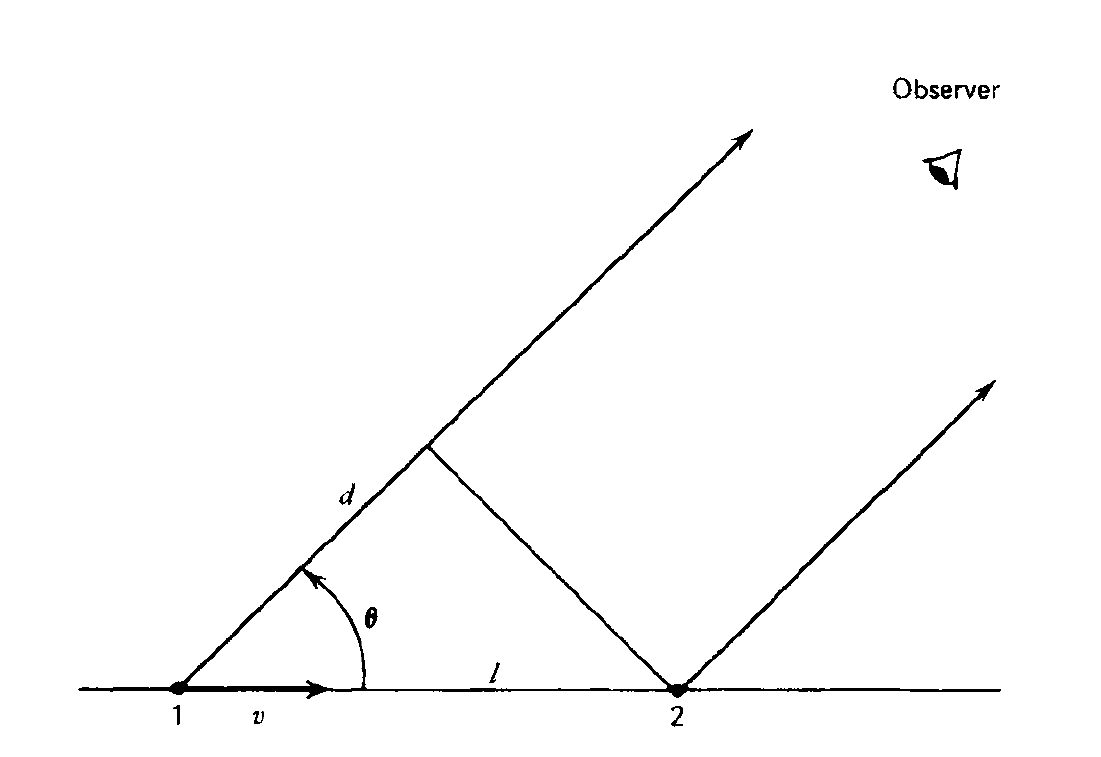
\includegraphics[scale= 0.2]{Figures/RelatDopplerGeometry.png}
 \caption{Γεωμετρία φαινομένου \textlatin{Doppler.} (Εικόνα \cite{1986rpa..book.....R}) }
 \label{fig:lightpathsphere}
 \end{center}
 \end{figure}
Άρα η ισχύς ανά στερεά γωνία  που εκπέμπεται και η ισχύς ανά στερεά γωνία  που λαμβάνεται και καταγράφεται (στο σύστημα $Κ$) θα είναι, δεδομένου ότι $\mu^\prime = \frac{\mu-\beta}{1-\mu \beta}$:
\begin{subequations}
\label{eq:PowerSolAngle}
\begin{align}
\dfrac{dP_e}{d\Omega} = \dfrac{dW}{dt_e d\Omega} = \gamma^3(1+\beta \mu^\prime)^3\dfrac{dW^\prime}{\gamma dt_e^\prime  d\Omega^\prime} = \frac{1}{\gamma^4 (1-\beta\mu)^3}\dfrac{dP_e^\prime}{d\Omega^\prime}   \label{eq:PowerSolAngleA} \\ 
\dfrac{dP_r}{d\Omega} = \dfrac{dW}{dt_r d\Omega} = \gamma^3(1+\beta \mu^\prime)^3\dfrac{dW^\prime}{\gamma (1-\beta \mu) dt_r^\prime  d\Omega^\prime} = \frac{1}{\gamma^4 (1-\beta\mu)^4}\dfrac{dP_r^\prime}{d\Omega^\prime}   \label{eq:PowerSolAngleB} 
\end{align}
\end{subequations}
Η ισχύς ακτινοβολίας που εκπέμπεται ανά στερεά γωνία δίνεται από την εξίσωση \ref{eq:PowerSolAngleA} ενώ η ισχύς ακτινοβολίας ανά στερεά γωνία που παρατηρείται δίνεται από την εξίσωση \ref{eq:PowerSolAngleB}\cite{1986rpa..book.....R}. Οι δύο αυτές σχέσεις, όπως βλέπουμε, διαφοροποιούνται. Όταν μιλάμε για παρατηρήσεις αστροφυσικών αντικειμένων ως ισχύ ακτινοβολίας εννοούμε την παρατηρούμενη- εκτός αν επισημανθεί διαφορετικά.
%============================================================
%============================================================
%============================================================

\section{Βασικές έννοιες ακτινοβολίας}
Για να περιγράψουμε την αλληλεπίδραση ακτινοβολίας με την ύλη χρησιμοποιούμε τρείς βασικές ποσότητες: 
\begin{itemize}
    \item την ειδική ένταση ακτινοβολίας $I_\nu$ που μας δίνει την τοπική ροή ανά μονάδα χρόνου, συχνότητας, επιφάνειας και στερεάς γωνίας στην πηγή 
    \item τον συντελεστή μονοχρωματικής απορρόφησης $\kappa_\nu$  που συνδυάζει όλες τις διαδικασίες απώλειας ενέργειας (απορρόφηση  και σκεδασμό)
    \item τον συντελεστή μονοχρωματικής εκπομπής $j_\nu$ που δίνει την τοπικά εκπεμπόμενη ροή ανά μονάδα όγκου, χρόνου, συχνότητας και στερεάς γωνίας
\end{itemize}      
Οι παραπάνω ποσότητες συνθέτουν την εξίσωση διάδοσης ακτινοβολίας 
\begin{equation}
    \frac{dI_\nu}{ds} = -\kappa_\nu I_\nu+j_\nu
\end{equation}
όπου $ds$ είναι το στοιχείο μήκους, ο πρώτος όρος του δεξιού μέλους περιγράφει την απώλεια ενέργειας λόγω απορρόφησης και ο δεύτερος περιγράφει την παραγωγή ακτινοβολίας από διαδικασίες εκπομπής\cite{netzer_2013}. Ορίζουμε το στοιχείο οπτικού βάθους $d \tau_\nu = \kappa_\nu ds$ και η παραπάνω εξίσωση γίνεται
\begin{equation}
    \frac{dI_\nu}{d\tau_\nu} = -I_\nu+S_\nu
\end{equation}
Η συνάρτηση $S_\nu =j_\nu/\kappa_\nu $ λέγεται συνάρτηση πηγής. Η γενική εξίσωση διάδοσης ακτινοβολίας είναι περίπλοκη και απαιτεί αριθμητικές τεχνικές για την λύση της. Ωστόσο, για περιπτώσεις απλής γεωμετρίας και κατακόρυφης διεύθυνσης η αναλυτική λύση εξάγεται εύκολα\cite{netzer_2013}.
%============================================================
%============================================================
%============================================================

\section{Ακτινοβολία σύγχροτρον}

Σύμφωνα με την σύγχρονη φυσική κατανόηση των ενεργών γαλαξιακάων πυρήνων, θεωρείται ότι το μεγαλύτερο ποσό της συνολικής μη-θερμικής ακτινοβολίας των \textlatin{AGN} οφείλεται σε εκπομπή ακτινοβολίας σύγχροτρον. Η ακτινοβολία σύγχροτρον σχετίζεται με την ραδιοεκπομπή των ενεργών γαλαξιακών πυρήνων.

\subsection*{Εκπομπή ενός ηλεκτρονίου σε μαγνητικό πεδίο}

Για ηλεκτρόνιο ενέργειας $E$ που κινείται σε ομοιογενές μαγνητικό πεδίο $B$ πυκνότητας ενέργειας $u_B = B^2/8\pi$ ο ρυθμός απώλειας ενέργειας $-dE/dt$ είναι ακριβώς η ισχύς $P$ που εκπέμπεται από το ηλεκτρόνιο δίνεται από την σχέση\cite{netzer_2013} 
\begin{equation}
    P = 2\sigma_T c \gamma^2\beta^2u_Bsin^2\alpha
\end{equation}
όπου $\sigma_T$ η διατομή \textlatin{Thomson}, $c$ η ταχύτητα του φωτός στο κενό, $\gamma = E/m_e c^2$ o παράγοντας \textlatin{Lorentz} kai $\beta=v/c$, όπου $v$ η ταχύτητα του ηλεκτρονίου. Ο όρος $sin^2\alpha$ αναπαριστά την διεύθυνση κίνησης, με $\alpha$ την οξεία γωνία που σχηματίζει η διεύθυνση κίνησης με το μαγνητικό πεδίο. Ο μέσος όρος για ισοτροπικές οξείες γωνίες\cite{netzer_2013}
\begin{equation}
    \overline{P} = \frac{4}{3} \sigma_T c \gamma^2\beta^2u_B \label{eq:powerSynch} 
\end{equation}
Η ακτινοβολία από ένα ηλεκτρόνιο εκπέμπεται στην διεύθυνση της κίνησης. Η κατανομή φασματικής ενέργειας (\textlatin{SED}) της ακτινοβολίας αυτής υπολογίζεται λαμβάνοντας υπ>όψιν την γυροσυχνότητα των ηλεκτρονίων γύρω από τις δυναμικές γραμμές του μαγνητικού πεδίου ($\omega_B = eB/\gamma m_e c$) και το μέσο διάστημα μεταξύ παλμών ($2\pi /\omega_B$). Το πλάτος του παλμού υπολογίζεται λαμβάνοντας υπ>όψιν τον σχετικιστικό μετασχηματισμό χρόνου μεταξύ του αδρανειακού συστήματος ηρεμίας του ηλεκτρονίου και το αδρανειακό σύστημα παρατήρησης, έτσι το πλάτος του παλμού είναι ανάλογο του $\gamma^{-3}$. O μετασχηματισμός \textlatin{Fourier} του παλμού, μας δίνει το μέσο εκπεμπόμενο φάσμα ενός ηλεκτρονίου $\overline{P_\nu}(\gamma)$ το οποίο έχει μέγιστο κοντά στο $\gamma \omega_L$, όπου $\omega_L$ η συχνότητα \textlatin{Larmor} με $\omega_L = eB/m_ec$ \cite{netzer_2013}.

\subsection*{Εκπομπή σύγχροτρον από κατανομή ηλεκτρονίων νόμου δύναμης}

Θεωρούμε συλλογή ηλεκτρονίων με κατανομή ενεργειών $n(\gamma)d\gamma$ η οποία μας δίνει το πλήθος των ηλεκτρονίών ανά μονάδα όγκου με ταχύτητες τέτοιες ώστε η τιμή της παραμέτρου $\gamma$ να βρίσκεται στο διάστημα $\gamma - (\gamma +d\gamma)$. Ο συντελεστής εκπομπής των ηλεκτρονίων για όλες τις ενέργειες θα είναι\cite{netzer_2013}
\begin{equation}
    j_\nu =\frac{1}{4\pi} \int_1^\infty \overline{P_\nu}(\gamma) n(\gamma)d\gamma 
\end{equation}
Το παραπάνω ολοκλήρωμα δεν έχει γενική λύση, αφού η κατανομή ενεργειών $n(\gamma)$ μπορεί να πάρει οποιαδήποτε μορφή, όμως υπάρχουν περιπτώσεις όπου η $n(\gamma)$ περιγράφεται ως νόμος δύναμης στις ενέργειες $n(\gamma )d\gamma = n_0 \gamma^{ − p} d\gamma $. Επίσης, κάνοντας την παραδοχή ότι κάθε ακτινοβολία έχει ένα μέγιστο κοντά σε μία χαρακτηριστική συχνότητα $\gamma^2 \nu_L$, όπου $\nu_L$ η συχνότητα \textlatin{Larmor}, προκύπτει η αναλυτική μορφή του συντελεστή εκπομπής\cite{netzer_2013}
\begin{equation}
    4\pi j_\nu =\frac{2}{3} \sigma_T n_0 u_B \nu_L^{-1} \Big( \frac{\nu}{\nu_L} \Big)^{-\frac{p-1}{2}}
\end{equation}
Η μονοχρωματική φωτεινότητα $L_\nu$ οπτικά αραιού μέσου που εκπέμπει ακτινοβολία σύνχροτρον προκύπτει ολοκληρώνοντας τον παράγοντα εκπομπής στον όγκο της πηγής\cite{netzer_2013}
\begin{equation}
    L_\nu =\int_V j_\nu dV  \propto \nu^{-\frac{p-1}{2}} \label{eq:LumiSynch}
\end{equation}
Η λογαριθμική κλίση προσαρμόζεται στο παρατηρούμενο φάσμα πολλών \textlatin{AGN} στα ραδιοκύματα, στο οπτικό/υπεριώδες και στις ακτίνες Χ. 

\subsection*{Αυτοαπορρόφηση σύγχροτρον}

Η εκπομπή σύγχροτρον συνοδεύεται από απορρόφηση, κατά την οποία ένα φωτόνιο αλληλεπιδρά με φορτίο εντός του μαγνητικού πεδίου και απορροφάται αποδίδοντας όλη του την ενέργεια στο φορτίο. Μία άλλη διαδικασία που μπορεί να συμβεί είναι η εξαναγκασμένη εκπομπή ή αρνητική απορρόφηση, κατά την οποία ένα σωματίδιο εκπέμπει ισχυρότερα σε μία συχνότητα\cite{1986rpa..book.....R}. Ο συντελεστής αυτοαπορρόφησης σύγχροτρον προκύπτει\cite{1986rpa..book.....R} $\alpha_\nu \propto \nu^{-(p+4)/2} $.
%============================================================
%============================================================
%============================================================

\section{Σκεδασμός \textlatin{Compton}}

Η αλληλεπίδραση ηλεκτρόνιου με δέσμη φωτονίου περιγράφεται από τον σκεδασμό \textlatin{Compton}. Για στατικά ή αργά κινούμενα ηλεκτρόνια, χρησιμοποιούμε τις σχέσεις διατήρησης ενέργειας και ορμής για να εξάγουμε τις σχέσεις μεταξύ των συχνοτήτων της προσπίπτουσας δέσμης φωτονίων ($\nu^\prime$) και της σκεδαζόμενης δέσμης φωτονίων ($\nu$). Αν $\vec{n_\nu}$ και $\vec{n_{\nu^\prime}}$ μοναδιαία διανύσματα στις διευθύνσεις των δέσμων αυτών και γωνία $\theta$ τέτοια ώστε $cos \theta = \vec{n_\nu} \cdot \vec{n_{\nu^\prime}} $, τότε\cite{netzer_2013}
\begin{equation}
    \nu =\dfrac{ m_e c^2\; \nu^\prime }  { m_e c^2+ h \nu^\prime(1-cos\theta) } \label{eq:ComptonWavelength} 
\end{equation}
Για μη σχετικιστικά ηλεκτρόνια η ενεργός διατομή της διαδικασίας αυτής δίνεται από την εξίσωση\cite{netzer_2013}
\begin{equation}
    \frac{d\sigma}{d\Omega} =\frac{1}{2}  r_e^2 (1+cos^2 \theta)
\end{equation}
όπου $r_e = e^2/m_e c^2$ η ακτίνα ηλεκτρονίου στην κλασσική φυσική. Η ολοκλήρωση της παραπάνω σχέσης σε όλες τις γωνίες μας δίνει την ενεργό διατομή \textlatin{Thomson} $\sigma_T$.\\
Στο όριο των υψηλών ενεργειών χρησιμοποιούμε την ενεργό διατομή \textlatin{Klein–Nishina} $\sigma_{KN}$ για την έκφραση της οποίας χρησιμοποιούμε την ποσότητα $\epsilon = h\nu/m_e c^2$ οπότε η προσέγγιση γίνεται\cite{netzer_2013} 
\begin{equation}
    \sigma_{KN} =\begin{cases} \sim \sigma_T (1-2\epsilon)\;\;\;\;\;\;\;\; \;\;\;\;\;\;\; \mbox{gia}\;\; \epsilon<<1 
    \\ \;\\ 
    \sim \frac{3}{8}\frac{\sigma_T}{\epsilon} \Big(ln2\epsilon +\frac{1}{2} \Big) \;\;\;\;\;\;\;\; \mbox{gia}\;\; \epsilon>>1 \end{cases}
\end{equation}

\subsection*{Αντίστροφος σκεδασμός \textlatin{Compton}}

Ο αντίστροφος σκεδασμός \textlatin{Compton} είναι η διαδικασία κατά την οποία (σχετικιστικά) κινούμενο ηλεκτρόνιο σκεδάζει φωτόνιο, με αποτέλεσμα να του μεταφέρει μέρος της ενέργειάς του. Μας ενδιαφέρει η εξίσωση για την μέση ισχύ που εκπέμπεται λόγω αντιστρόφου σκεδασμού \textlatin{Compton} για κατανομή φωτονίων που σκεδάζονται από μια δεδομένη ισοτροπική κατανομή κινούμενων ηλεκτρονίων. Θεωρούμε αριθμητική πυκνότητα $n_{ph}$ δέσμης φωτονίων με μέση ενέργεια πριν την σκέδαση $h\overline{\nu_0}$. Η ενεργειακή πυκνότητα των φωτονίων αυτών θα είναι $u_{rad} = n_{ph} h\overline{\nu_0}$. Η μέση ενέργεια μετά την σκέδαση $h\overline{\nu}$, όπως φαίνεται από την σχέση \ref{eq:ComptonWavelength}, είναι μεγαλύτερη από αυτήν πριν την σκέδαση κατά παράγοντα τάξης $\gamma^2$. Στο σύστημα ηρεμίας του ηλεκτρονίου η διαδικασία αυτή μοιάζει με σκεδασμό \textlatin{Thomson} με μέση ισχύ ακτινοβολίας που δίνεται από την σχέση $\overline{P} = \sigma_T c u_{rad} $. Έτσι, για την απλή εκτίμηση $L_\nu \propto \nu^{-(p-1)/2}$, sto αδρανειακό σύστημα παρατήρησης η μέση εκπεμπόμενη ισχύς είναι $ \overline{P} = \gamma^2 \sigma_T c u_{rad} $. Ενώ ο ακριβής υπολογισμός της μέσης εκπεμπόμενης ισχύος λαμβάνει υπ>όψιν την γωνία σκέδασης και τον μετασχηματισμό της από το σύστημα ηρεμίας του ηλεκτρονίου στο σύστημα παρατήρησης και η τελική σχέση που προκύπτει είναι\cite{netzer_2013}
\begin{equation}
    \overline{P} = \frac{4}{3} \sigma_T c \gamma^2 \beta^2 u_{rad} \label{eq:powerIC} 
\end{equation}
Η έκφραση μέσης ακτινοβολούμενης ισχύος λόγω αντιστρόφου \textlatin{Compton} (εξίσωση \ref{eq:powerIC}) δεν διαφέρει σημαντικά από την έκφραση μέσης ακτινοβολούμενης ισχύος ακτινοβολίας σύγχροτρον (εξίσωση \ref{eq:powerSynch}). Η μόνη διαφορά έγκειται στο ότι η ενεργειακή πυκνότητα του μαγνητικού πεδίου $u_B$ της εξίσωσης για την ακτινοβολία σύγχροτρον αντικαθίσταται στην αντίστοιχη σχέση αντιστρόφου \textlatin{Compton} με την ενεργειακή πυκνότητα του πεδίου ακτινοβολίας $u_{rad}$. Οπότε, θεωρώντας ότι αυτές οι δύο διαδικασίες λαμβάνουν χώρα στον ίδιο όγκο, η μέση ισχύς ακτινοβολίας τους θα είναι $u_B/u_{rad}$. Η κατανομή ενέργειας των σχετικιστικών ηλεκτρονίων στο ίδιο αυτόν όγκο δίνεται από την ίδια συνάρτηση νόμου δύναμης που χρησιμοποιήθηκε στην περίπτωση της ακτινοβολίας σύγχροτρον $n(\gamma) \propto \gamma^{-p}$ με αποτέλεσμα να έχουμε την ίδια εξάρτηση της μονοχρωματικής φωτεινότητας από την παράμετρο $p$\cite{netzer_2013} 
\begin{equation}
    L_\nu \propto \nu^{-\frac{p-1}{2}} \label{eq:LumiIC} 
\end{equation}

\subsection*{Μηχανισμός \textlatin{Synchrotron-Self-Compton}}

Σε συμπαγή πηγή ακτινοβολίας σύγχροτρον τα εκπεμπόμενα φωτόνια μπορούν μέσω αντιστρόφου \textlatin{Compton} να σκεδαστούν από τα ίδια σχετικιστικά ηλεκτρόνια που εκπέμπουν την ακτινοβολία σύγχροτρον. Η διαδικασία αυτή αυξάνει σημαντικά την ενέργεια του φωτονίου και η ακτινοβολία που προκύπτει ονομάζεται εκπομπή \textlatin{Synchrotron-Self-Compton (SSC)}. Ο μηχανισμός αυτός αφορά ακτινοβολίες πολύ υψηλών ενεργειών (ακτίνες $\gamma$ από $>100$ \textlatin{MeV} έως τάξης \textlatin{ΤeV}) από ραδιογαλαξίες, \textlatin{pulsar} ή υπερκαινοφανείς. Η ροή που εκπέμπεται από την διαδικασία αυτή υπολογίζεται ολοκληρώνοντας το φάσμα της ακτινοβολίας σύγχροτρον και την κατανομή ενέργειας του πεδίου ηλεκτρονίων. Σε καλή προσέγγιση ο φασματικός δείκτης (λογαριθμική κλίση) που προκύπτει είναι συμβατός με τον φασματικό δέικτη της πηγής σύγχροτρον.\\
Η διαδικασία \textlatin{Synchrotron-Self-Compton} μπορεί να επαναλαμβάνεται στην ίδια πηγή από περεταίρω σκέδαση των παραγόμενων φωτονίων, με αποτέλεσμα να αυξάνεται η ενέρεγια των φωτονίων κατά παράγοντα $\gamma^2$. Το φυσικό όριο της διαδικασίας αυτής έρχεται όταν η ενέργεια σκεδαζόμενου φωτονίου αγγίζει το φάσμα των ακτίνων $\gamma$ και η συνθήκη $h \nu_\gamma \ll m_e C^2 $ για μη-ανάκρουση \textlatin{Compton} των ηλεκτρονίων παύει να ισχύει, στο όριο αυτό η πυκνότητα ακτινοβολίας ελαττώνεται γρήγορα\cite{netzer_2013}.\\
Ο μηχανισμός αυτός παράγει την ακτινοβολία Χ που παρατηρούμε σε ενεργούς γαλαξιακούς πυρήνες και παράγεται από διαδικασίες που σχετίζονται άμεσα με την προσάυξηση μάζας στην κεντρική μελανή οπή.

%============================================================
%============================================================
%============================================================

\section{Ακτινοβολία πέδης (\textlatin{bremsstrahlung})}

Η ακτινοβολία λόγω επιτάχυνσης φορτίου σε πεδίο \textlatin{Coulomb} που παράγει άλλο φορτίο λέγεται ακτινοβολία πέδης, ή \textlatin{bremsstrahlung}, ή εκπομπή \textlatin{free-free}.\\
H ακτινοβολία \textlatin{bremsstrahlung} από σύγκρουση όμοιων σωαμτιδίων (π.χ. ηλεκτρονίου-ηλεκτρονίου) δίνει μηδενική ένταση ακτινοβολίας στην προσέγγυση διπόλου, οπότε μας ενδιαφέρει η σύγκρουση διαφορετικών σωματιδίων. Ακτινοβολία \textlatin{bremsstrahlung} μελετάμε κυρίως από ζέυγος ηλεκτρονίου-ιόντος, αφού η σχετικές επιταχύνσεις τους είναι αντιστρόφως ανάλογες των μαζών και τα φορτία τους σχεδόν ίσα. Η μάζα του ιόντος είναι κατά πολλύ μεγαλύτερη αυτής του ηλεκτρονίου, οπότε μπορούμε να μελετάμε το ηλεκτρόνιο σαν να κινείται σε σταθερό πεδίο  \textlatin{Coulomb} του ιόντος\cite{1986rpa..book.....R}.\\
Η ακτινοβολία \textlatin{bremsstrahlung} είναι τεχνικά θερμική ακτινοβολία, όμως το σχήμα του φάσματος διαφέρει από αυτό μελανού σώματος. Η εκπομπή ακτινοβολίας \textlatin{bremsstrahlung} από επιτάχυνση ηλεκτρονίου στο πεδίο ιόντος φορτίου $Z$ με αριθμητική πυκνότητα $N_i$ περιγράφεται από τον συντελεστή εκπομπής\cite{netzer_2013}
\begin{equation}
    4\pi j_\nu = 6.8\times 10^{-38} Z^2 T_e^{-1/2}N_e N_i g_{ff}(\nu, T_e,Z)e^{-h\nu/kT_e} 
\end{equation}
όπου $N_e$ kai $T_e$ η αριθμητική πυκνότητα και η θερμοκτρασία ηλεκτρονίων και $g_{ff}(\nu, T_e,Z)$ είναι η μέση τιμή του παράγοντα \textlatin{Gaunt} για όλες τις ταχύτητες- ο οποίος διορθώνει για κβαντικά φαινόμενα. Ο παράγοντας αυτός είναι τάξης $1$ και μπορεί να αλλάξει ελαφρώς με την συχνότητα. Για ενέργειες ακτίνων Χ έχουμε $g_{ff} \propto \nu^{-0.1}$. H ακτινοβολία \textlatin{bremsstrahlung} εκτείνεται σε πολλές διαφορετικές ενέργειες και το φάσμα της έχει μορφή νόμου δύναμης με πολύ μικρό φασματικό δέικτη (σχεδόν επίπεδο φάσμα)\cite{netzer_2013} σχετίζεται με εκπομπή ακτίνων Χ από σμήνη γαλαξιών στο συνεχές, αλλά και με εκπομπή γραμμών στα ραδιοκύματα από ιονισμένο υδρογόνο.\\
Ολοκληρώνοντας την εκπομπή σε όλες τις συχνότητες καταλήγουμε στην ολική ενέργεια ανά μονάδα ανά μονάδα όγκου ανά δευτερόλεπτο $C_{ff}$, η ποσότητα αυτή αναπαριστά επίσης τον ρυθμό ψύξης λόγω ακτινοβολίας πέδης. Η ολοκλήρωση αυτή δίνει\cite{netzer_2013}
\begin{equation}
    C_{ff} = 1.42\times 10^{-27} Z^2 T_e^{-1/2}N_e N_i g_{ff} \; erg \;s^{−1}\; cm^{−3}
\end{equation}
όπου η ποσότητα $g_{ff}$ εκφράζει την μέση τιμή για συχνότητες της μέσης τιμής για ταχύτητες του παράγοντα \textlatin{Gaunt} και απ'ιρνει τιμές $1.1-1.5$ \cite{netzer_2013}.
%============================================================
%============================================================
%============================================================ 

\section{Αστροφυσικές παρατηρήσεις \textlatin{AGN} στις ακτίνες Χ}
% Η πλεον ισχυση γραμμη εκπομπης στις ακτινες, Fe-Ka, εμφανιοζεται (μερικες φορες) φαρδυα λογω βρατυρικων φαινομενων και οχι επειδη προερχεται απο περιστρεφομενα νεφη γυρω απο τη μελανη οπη.
\begin{figure*}
 \begin{center}
 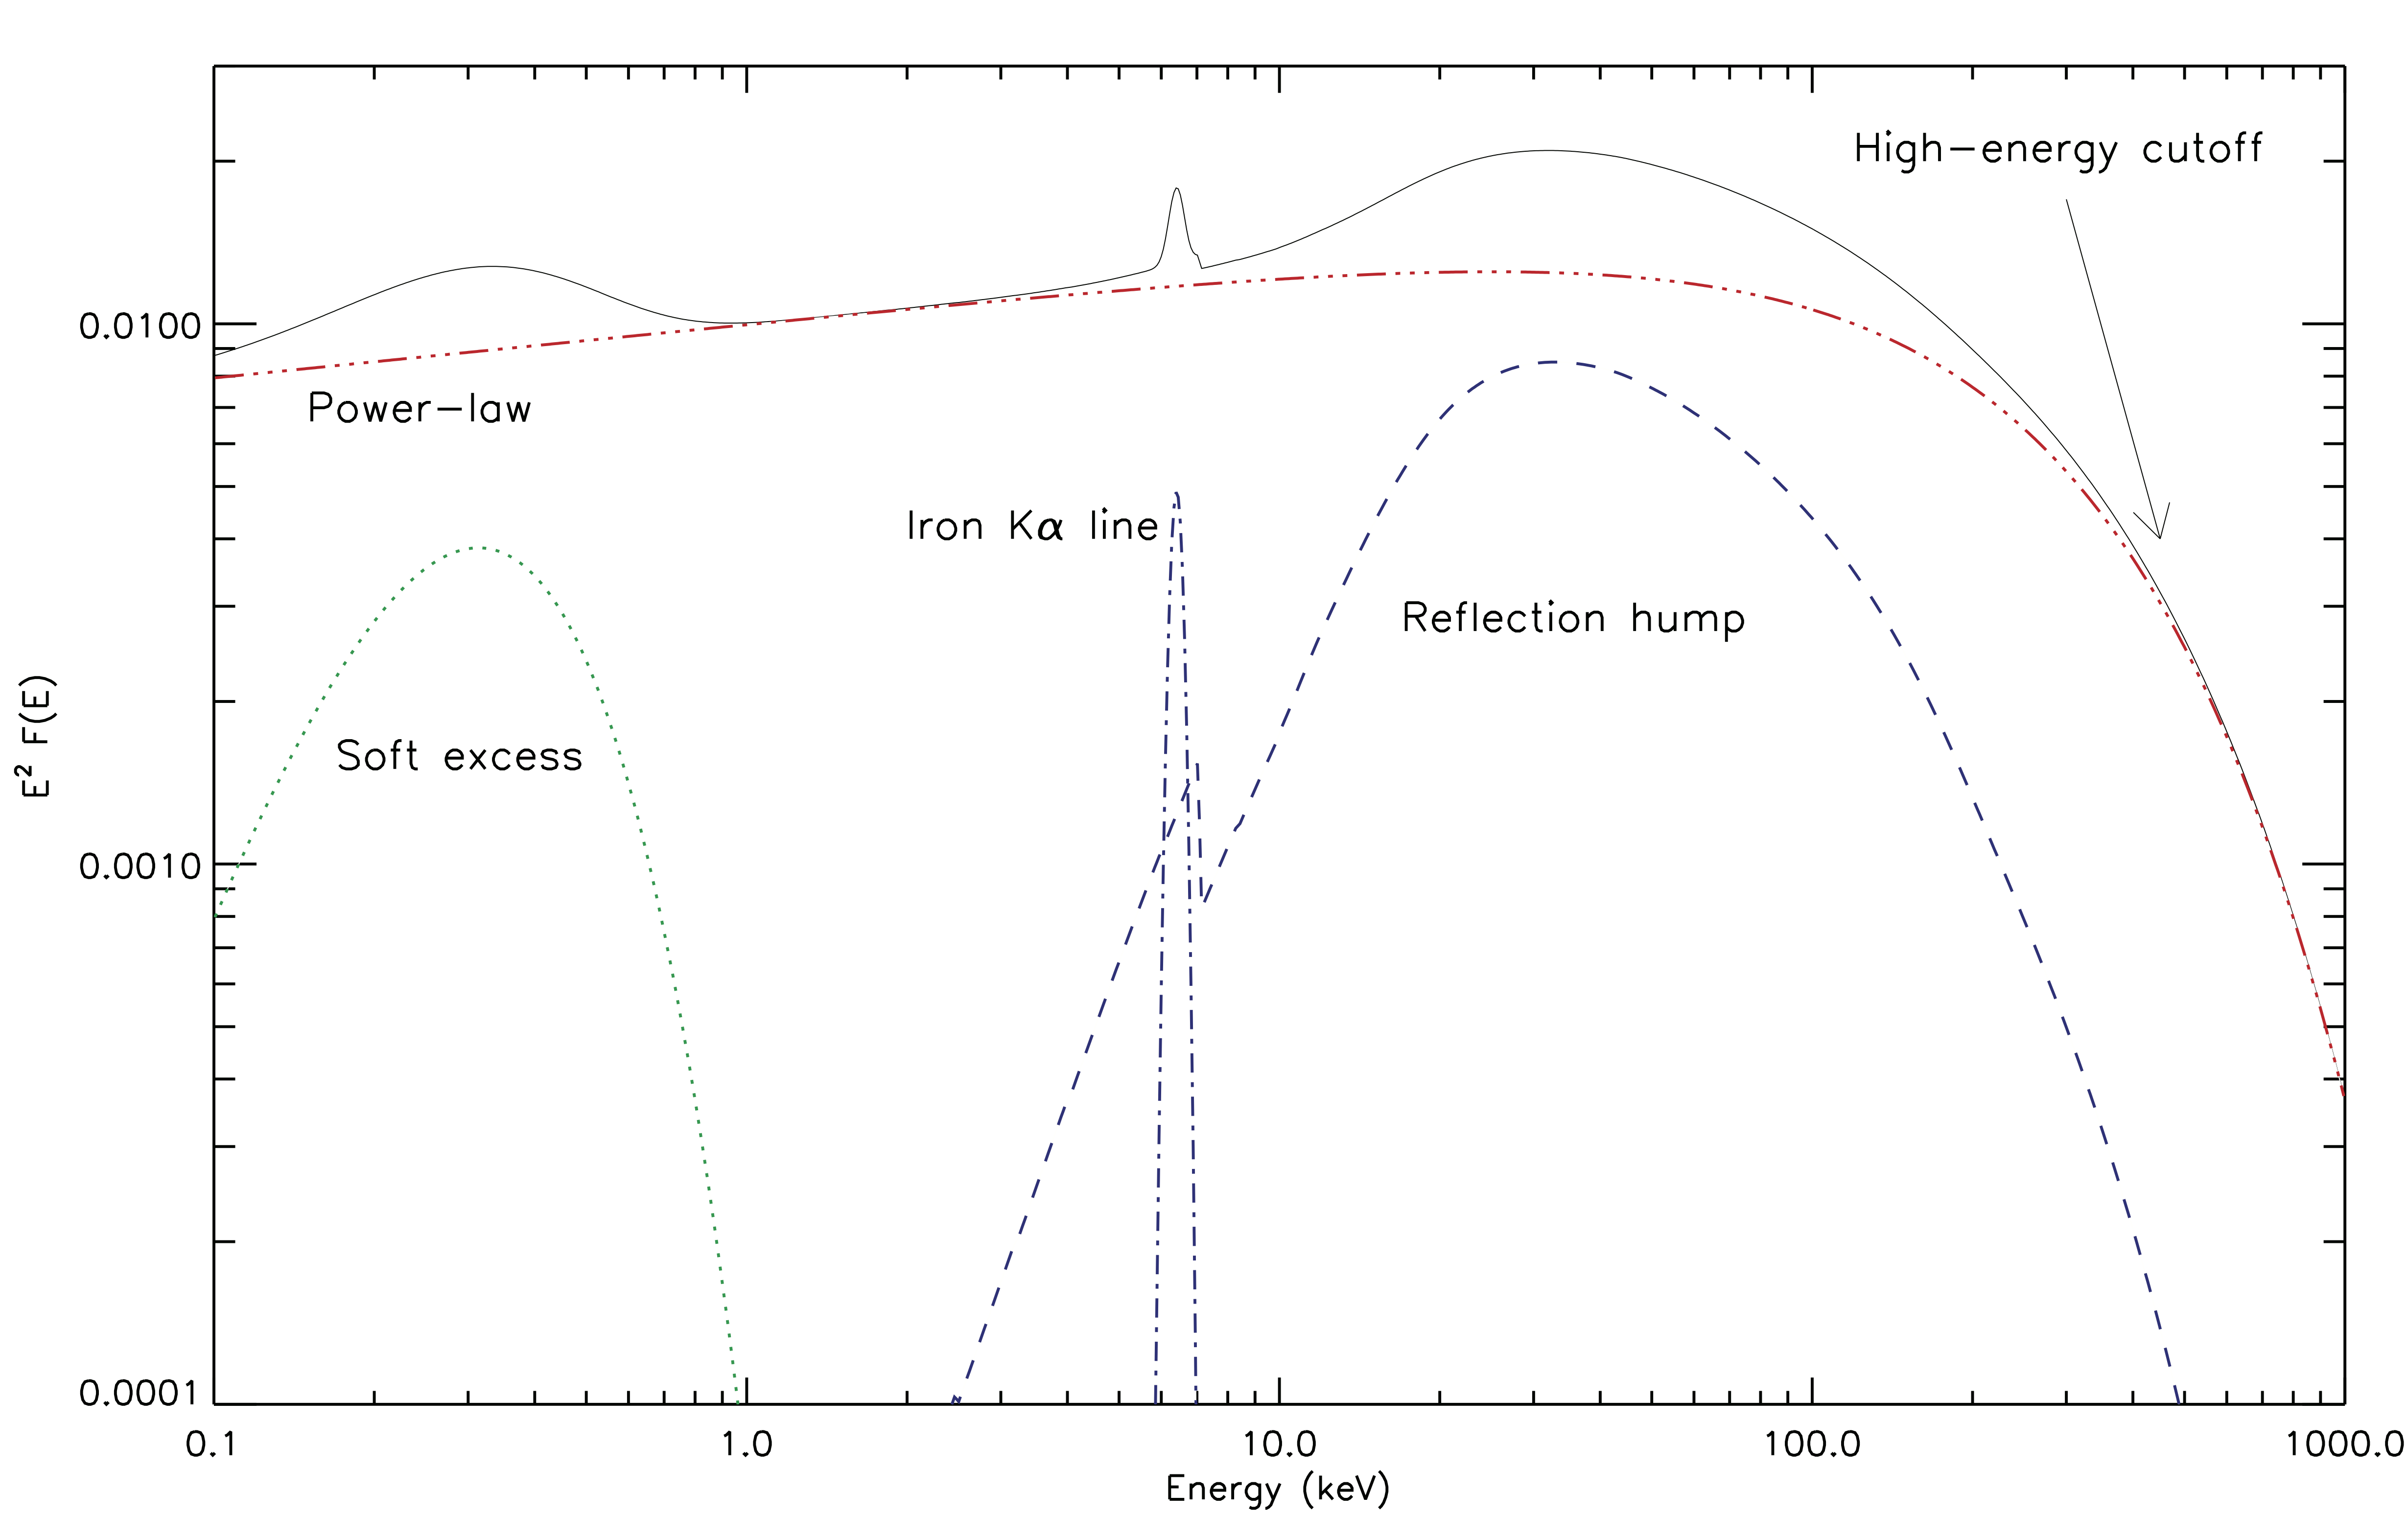
\includegraphics[width=0.9\linewidth]{Figures/X-ray_spectrum_AGN_hres.jpg}
 \caption{Τυπικό φάσμα \textlatin{AGN} τύπου 1 σε ενέργειες $0.1-1000$ \textlatin{keV} (Εικόνα από \textlatin{Ricci et al. 2011})} \label{fig:agnspec}
 \end{center}
\end{figure*}
Τα φάσματα των \textlatin{AGN} στις ακτίνες Χ είναι σχετικά ομοιογενή και περιγράφονται καλά με νόμο δύναμης μέσα σε ένα εύρος φασματικών δεικτών. Η γραμμή εκπομπής σιδήρου \textlatin{Fe K$_\alpha$} και η κύρτωση στα $\sim 10$ \textlatin{keV} θεωρείται ότι ωφείλονται σε ψυχρή ύλη (εικόνα \ref{fig:agnspec}). Μέρος της ψυχρής αυτής ύλης πρέπει να βρίσκεται κοντά στην περιοχή παραγωγής ακτίνων Χ, όπως υποδεικνύει η μικρή χρονική καθυστέρηση μεταξύ της μεταβολής στην γραμμή σε σχέση με την μεταβολή στο συνεχές. Η φυσική εξήγηση για την δομή είναι οπτικά πυκνός δίσκος προσάυξησης η εκπομπή από τον οποίο μπορεί να εξηγήσει το παρατηρούμενο φάσμα\cite{1991ApJ}.
\begin{figure*}
 \begin{center}
 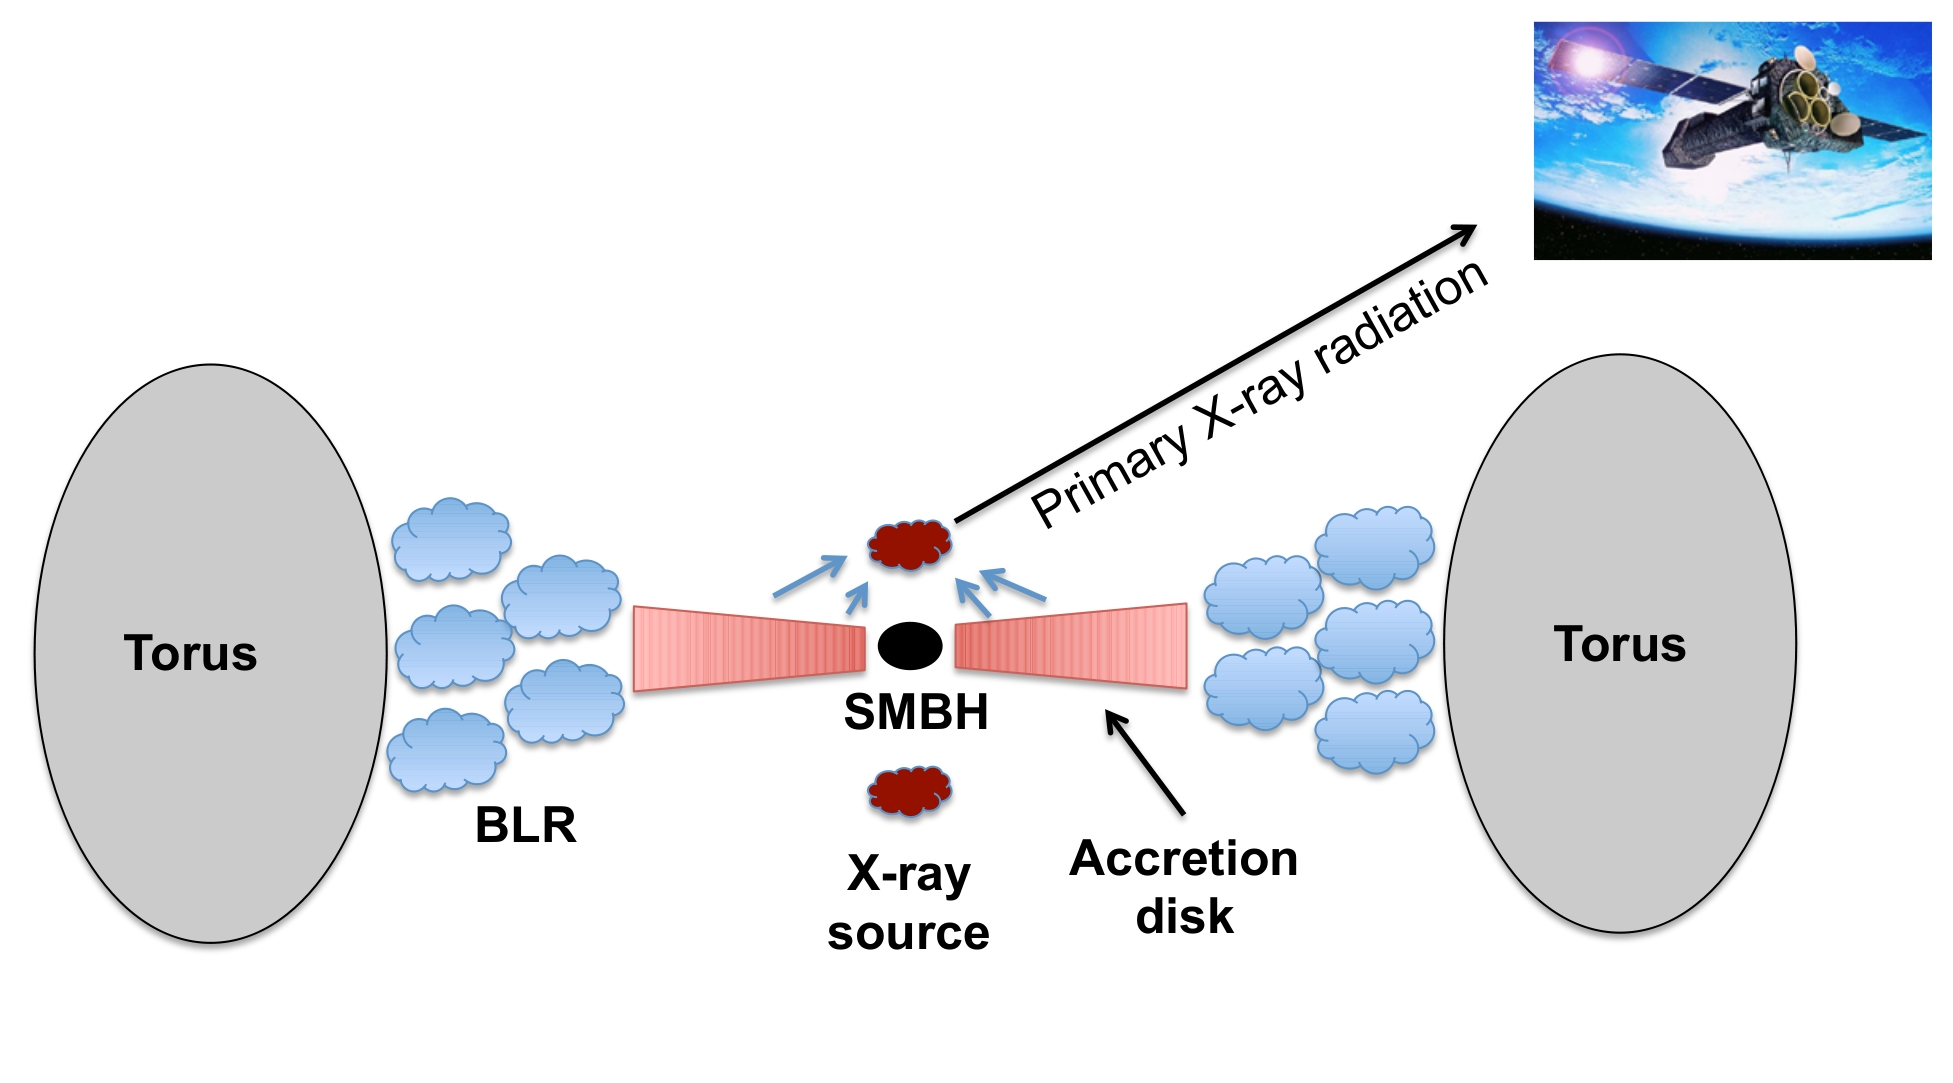
\includegraphics[width=0.7\linewidth]{Figures/X_ray_primary_1.jpg}
 
 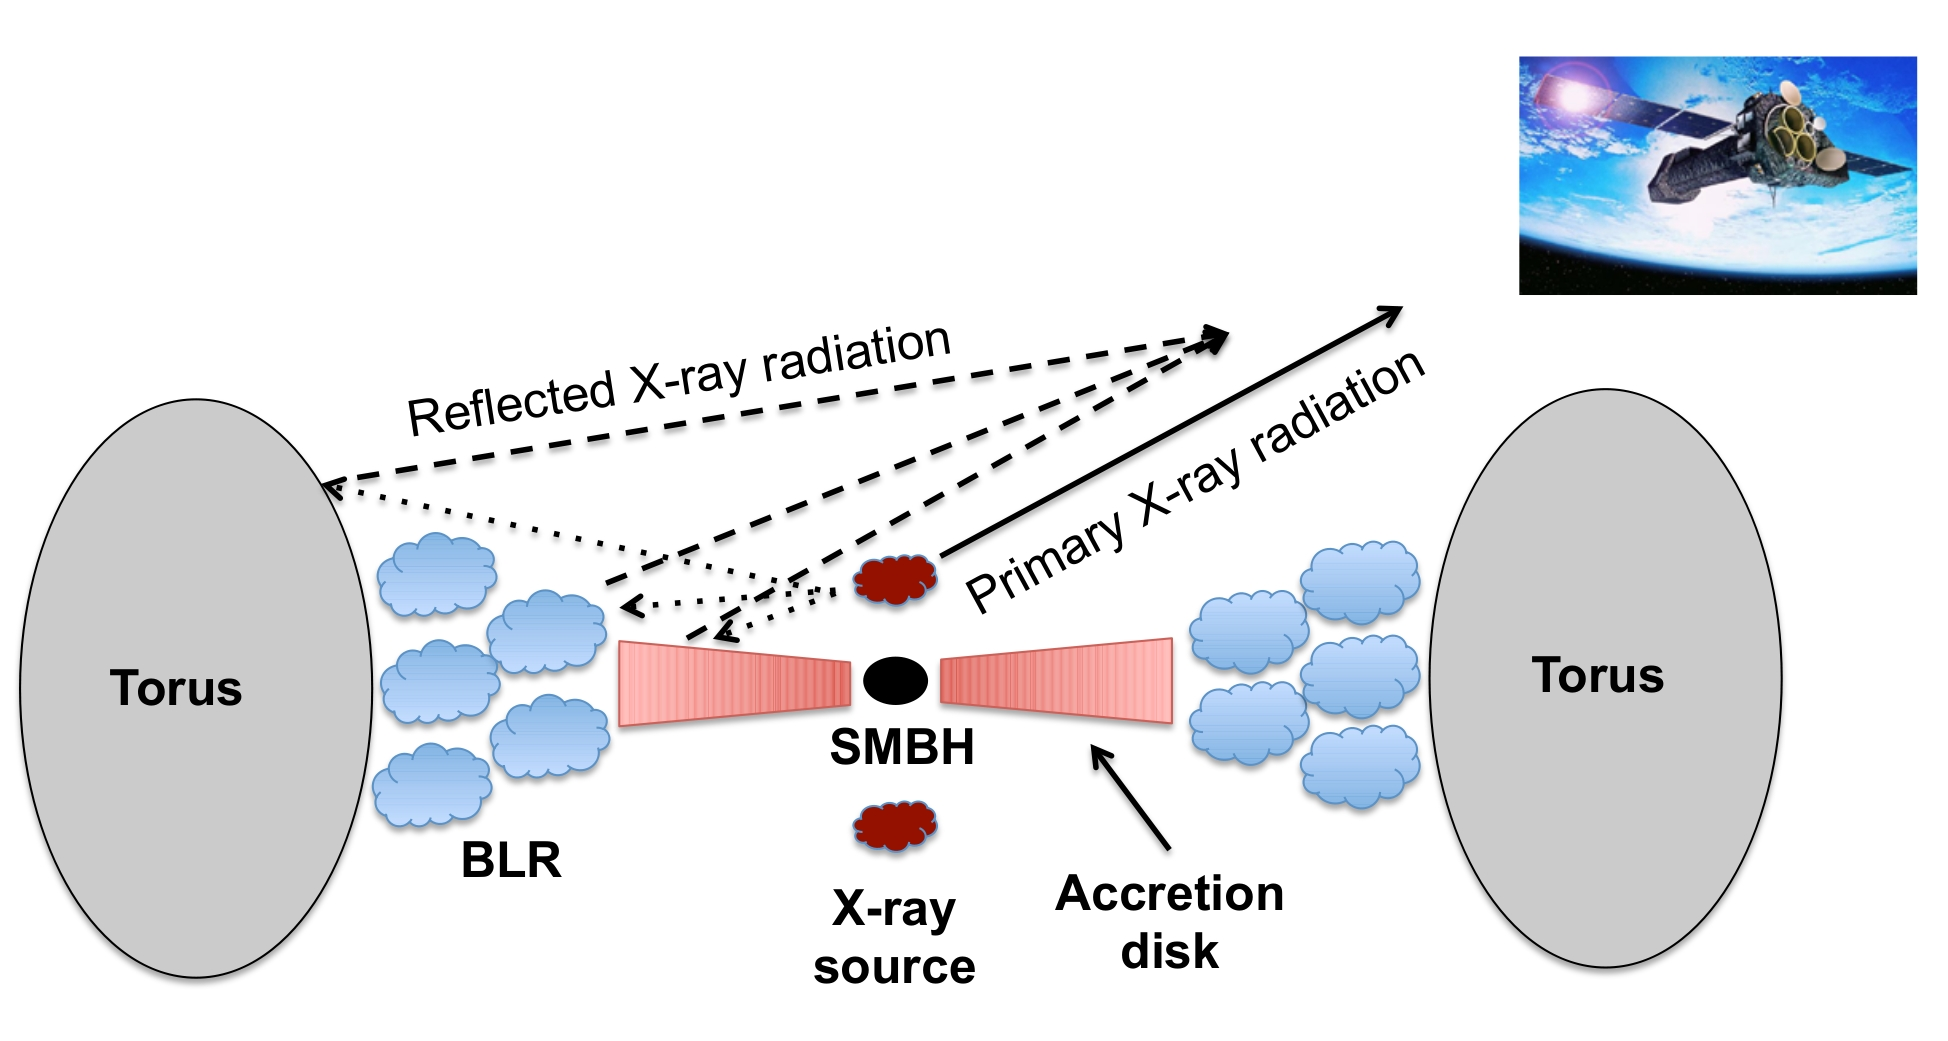
\includegraphics[width=0.7\linewidth]{Figures/X_ray_refl_1.jpg}
 \caption{Σχηματική αναπαράσταση παραγωγής ακτίνων Χ σε \textlatin{AGN}- η περιοχή από την οποία προέρχονται οι ακτίνες Χ είναι πιθανότατα ένα στέμμα πλάσματος ηλεκτρονίων. Πάνω: διαδρομή φωτός πρωτογενών ακτίνων Χ. Κάτω: διαδρομή φωτός δευτερογενών ακτίνων Χ (Εικόνα από \textlatin{www.isdc.unige.ch/$\sim$ricci})} \label{fig:xray_primary}
 \end{center}
\end{figure*}
Η αιτία που παράγει την μορφή νόμου δύναμης των φασμάτων των \textlatin{AGN} δεν είναι ξεκάθαρη. 
% Έχει εξετασθεί μοντέλο κατά το οποία κάποιος μηχανισμός εισάγει υψηλοενεργειακά φωτόνια που μετατρέπονται σε ζεύγος ηλεκτρονίου-ποζιτρονίου (παρουσία πυρήνα) και εκκινούν σωματιδιακούς καταιονισμούς που έχουν ως αποτέλεσμα διαδικασίες σκεδασμών \textlatin{Compton}. Άλλα μοντέλα προτείνουν θερμική ακτινοβολία \textlatin{bremsstrahlung}, η οποία θεωρείται ο μηχανισμός που παράγει την μεγαλύτερη εκπομπή ακτίνων Χ σε παρατηρήσεις σμηνών γαλαξιών και έχει φάσμα συμβατό με νόμο δύναμης\cite{1991ApJ}.

Το κυρίαρχο μοντέλο βασίζεται σε αντίστροφους σκεδασμούς \textlatin{Compton} μαλακών φωτονίων που ψύχουν θερμό αέριο ηλεκτρονίων, αυτό μας δίνει την εικόνα θερμού στέμματος θερμικών ηλεκτρονίων υψηλής ενέργειας (T$_{electron} \sim 10^9$  K) που ακτινοβολείται από φωτόνια οπτικού/υπεριώδους που παράγονται στον δίσκο και ψύχεται μέσω αντίστροφης σκέδασης \textlatin{Compton} κατά την οποία τα προσπίπτοντα φωτόνια αυξάνουν την ενέργειά τους και σκεδάζονται ως ακτινοβολία Χ (εικόνα \ref{fig:xray_primary}). Η αντίστροφη σκέδαση \textlatin{Compton} παράγει φυσικά φάσμα νόμου δύναμης (εξίσωση \ref{eq:LumiIC}) και ο παρατηρούμενος φασματικός δείκτης είναι $\Gamma \sim 1.8-2.0$ \cite{1991ApJ}.\\    
Το μοντέλο αυτό εξηγεί ότι η αποκοπή στην μορφή νόμου δύναμης (\textlatin{broken power law}) οφείλεται στο γεγονός ότι το στέμμα πλάσματος ηλεκτρονίων είναι θερμικό- δηλαδή τα ηλεκτόνια ακολουθούν κατανομή \textlatin{Maxwell}. Το ενεργειακό κατώφλι της δίδυμης γένεσης (παραγωγής ζεύγους ηλεκτρονίου-ποζιτρονίου από φωτόνιο παρουσία πυρήνα) είναι $\sim 511$ \textlatin{keV}, οπότε το στέμμα πλάσματος έχει όριο θερμοκρασίας. Συγκεκριμένα, το στέμμα δεν μπορεί να σκεδάζει φωτόνια με ενέργεια πάνω από  $\sim 150$ \textlatin{keV} πολύ αποδοτικά- σε μεγαλύτερες ενέργειες αρχίζουν διαδικασίες δίδυμης γένεσης- έτσι έχουμε εκθετική αποκοπή στην ροή οποία συσχετίζεται με την θερμοκρασία του στέμματος. Οι ιδιότητες του στέμματος είναι χαοτικές και δεν μπορούν να υπολογιστούν από πρώτες αρχές\cite{Brandt}. \\
Μέρος της πρωταρχικής εκπομπής ακτίνων Χ που προκύπτει από αντίστροφο σκεδασμό \textlatin{Compton} προσπίπτει στον τόρο μοριακού αερίου, στην περιοχή εκπομπής διευρυμένων φασματικών γραμμών \textlatin{(Broad Line Region)} ή ακόμα και στον ίδιο τον δίσκο προσάυξησης (σχηματικά στην εικόνα \ref{fig:xray_primary}) και επανεκπέμπεται. Η επανεκπεμπόμενη ακτινοβολία είναι υπεύθυνη για την κύρτωση του φάσματος στις ενέργειες $\sim 30-40$ \textlatin{keV} (σχήμα \ref{fig:agnspec}) και την γραμμή εκπομπής σηδήρου \textlatin{Fe K$_\alpha$} στην ενέργεια $\sim 6.4 $ \textlatin{keV}. Η κύρτωση στα $\sim 30-40$ \textlatin{keV} σημειώνεται μόνο όταν το υλικό πρόσπτωσης είναι πυκνό (με πυκνότητα στήλης Ν$_{Η} >  1.5 \times  10^{24}$ \textlatin{cm}$^{-2}$ - η τιμή του ορίου αυτού αντιστοιχεί στο οπτικό βάθος για την σκέδαση \textlatin{Compton}), ενώ η γραμμή εκπομπής σηδήρου \textlatin{Fe $K_\alpha$} μπορεί να παραχθεί και σε αραιή ύλη και θεωρείται υπέρθεση εκπομπής μίας διευρυμένης γραμμής και μίας στενής γραμμής που υποδηλώνουν εκπομπή από μία εσωτερική περιοχή του συστήματος προσάυξησης (η διευρυμένη γραμμή- π.χ. προέρχεται από τον ίδιο τον δίσκο) και εκπομπή από μία μακρυνότερη περιοχή (η στενότερη γραμμή- π.χ. προέρχεται από τον τόρο ή την \textlatin{BLR}). Η διεύρυνση της γραμμής αυτής οφείλεται σε βαρυτικά φαινόμενα που είναι πιο έντονα στην περιοχή κοντά στην κεντρική μάζα.\\
Αρκετά φάσματα \textlatin{AGN} παρουσιάζουν πλεόνασμα ισχύος ακτινοβολίας που κυρτώνει ελαφρά τον νόμο δύναμης στα $\sim 2 $ \textlatin{keV} (σχήμα \ref{fig:agnspec}). Για τους \textlatin{AGN} τύπου 1 έχουν διατυπωθεί αρκετές πιθανές αιτίες για το πλεόνασμα μαλακών ακτίνων Χ όπως: ανάκλαση από ιονισμένο δίσκο, τοπική απορρόφηση από ιονισμένο άνεμο ή ύπαρξη ενός δεύτερου ψυχρότερου στέμματος. Στους \textlatin{AGN} τύπου 2 η περιοχή απορρόφησης επηρεάζει το παρατηρούμενο φάσμα ακτίνων Χ καθώς λαμβάνουν χώρα διαδικασίες όπως φωτοηλεκτρική απορρόφηση και σκεδασμός \textlatin{Compton}. Η φωτοηλεκτρική απορρόφηση γίνεται αισθητή για υλικό πυκνότητας στήλης N$_{H} \sim 10^{21}$ \textlatin{cm}$^{-2}$ εξαρτάται από την ενέργεια επηρεάζοντας τις μαλακές ακτίνες Χ περισσότερο ενώ δεν παίζει σημαντικό ρόλο για ακτινοβολία ενέργειας $> 10$ \textlatin{keV} για πυκνότητα στήλης N$_{H}<  10^{24}$ \textlatin{cm}$^{-2}$. Ο σκεδασμός \textlatin{Compton} γίνεται σημαντικός για υλικό απορρόφησης πυκνότητας N$_{H} \sim  10^{24}$ \textlatin{cm}$^{-2}$.

\section{\textlatin{XMM-Newton}}

Το διαστημικό παρατηρητήριο \textlatin{ΧΜΜ (X-ray Multi Mirror)} εκτοξεύθηκε τον Δεκέμβρη του 1999 και έχει τρία τηλεσκόπια ακτίνων Χ τύπου \textlatin{Wolter} τύπου 1 με διαφορετικούς ανιχνευτές ακτίνων Χ στο εστιακό τους κέντρο και ένα τηλεσκόπιο για οπτικό/υπεριώδες.

\subsection{Δομή τηλεσκοπίων ακτίνων Χ}

Η εστίαση των ακτίνων Χ δεν γίνεται με το ίδιο τρόπο όπως π.χ. στο οπτικό, καθώς οι ακτίνες Χ έχουν τόσο μικρό μήκος κύματος ώστε τείνουν να διαπερνούν τα κάτοπτρα για γωνία πρόσπτωσης (\textlatin{angle of incidence}) σχετικά μεγάλή\footnote{Εδώ όταν μιλάμε για γωνία πρόσπτωσης, θα εννοούμε την οξεία γωνία που σχηματίζει η δέσμη με την επιφάνεια πρόσπτωσης- και όχι με την κατακόρυφο σε αυτήν.}. Έτσι η τυπική δομή φακών και κατόπτρων που χρησιμοποιούνται για παρατηρήσεις στο οπτικό δεν χρησιμοποιούνται στην αστρονομία ακτίνων Χ. Όμως, για πολύ μικρές γωνίες πρόσπτωσης δηλαδή σχεδόν εφαπτομενική στην επιφάνεια πρόσπτωση (\textlatin{grazing incidence}) μια δέσμη ακτίνων Χ ανακλάται και συμπεριφέρεται όπως το οπτικό- όπως φαίνεται σχηματικά στο σχήμα \ref{fig:grazing_incidence}.

\begin{figure*}
 \begin{center}
 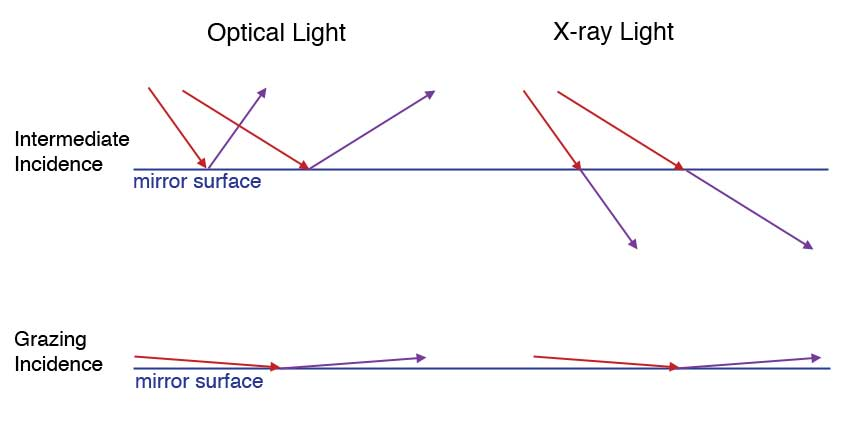
\includegraphics[width=0.7\linewidth]{Figures/grazing_incidence.jpg}
 \caption{Πάνω: πώς συμπεριφέρεται μια δέσμη οπτικού και μία δέσμη ακτίνων Χ κατά την πρόσπτωσή τους υπό μεσαία γωνία πάνω σε κάτοπτρο. Κάτω πώς συμπεριφέρονται οι ίδιες δέσμες για πρόσπτωση σχεδόν παράλληλη στην επιφάνεια- η γωνία που σχηματίζει η δέσμη με την επιφάνεια πρόσπτωσης στην περίπτωση της \textlatin{grazing incidence} για να ανακλαστεί η δέσμη ακτίνων Χ είναι στην πραγματικότητα μικρότερη από αυτήν που φαίνεται στο σχήμα. (Εικόνα από το <<\textlatin{Imagine the Universe}>> της \textlatin{NASA})}
 \label{fig:grazing_incidence}
 \end{center}
 \end{figure*}
  
\begin{figure*}
 \begin{center}
 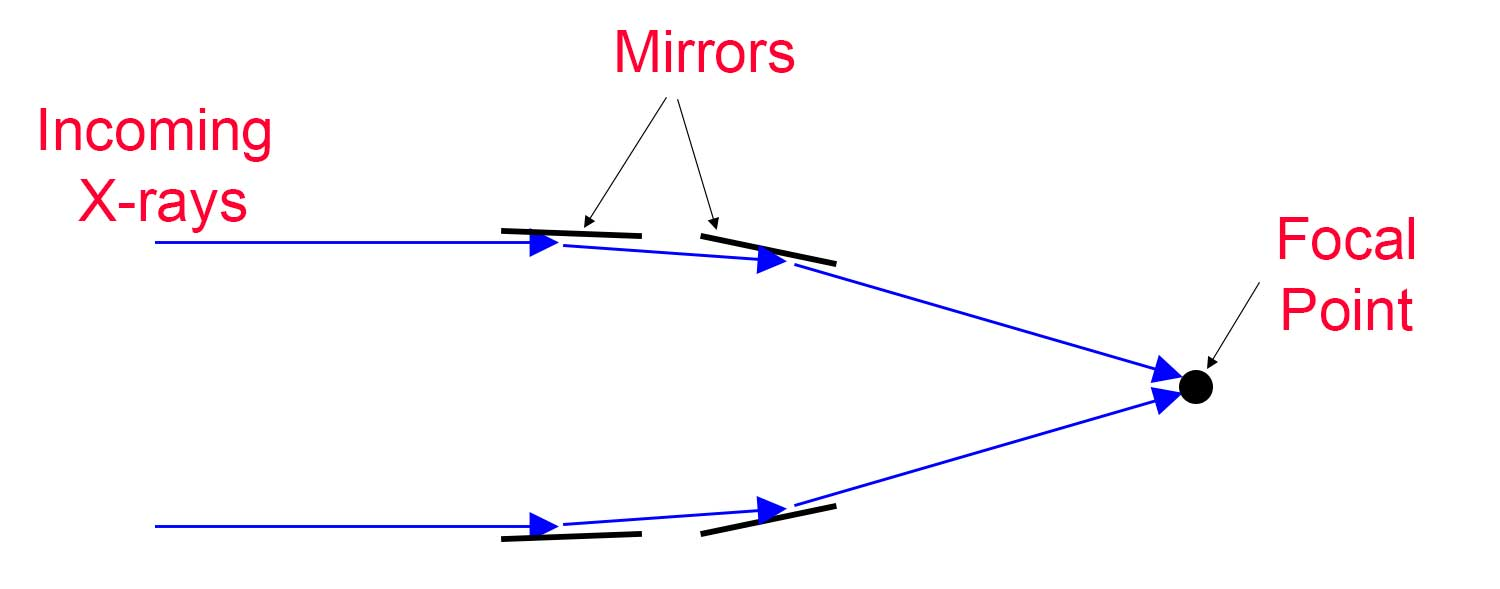
\includegraphics[width=0.7\linewidth]{Figures/xray_telescope_1mirror.jpg}
 \caption{Σχηματικό διάγραμμα κατά μήκος τομής τηλεσκοπίου ακτίνων Χ με ένα σετ κατόπτρων. Στο σχήμα με μπλε βέλη αναπαριστώνται εισερχόμενες ακτίνες Χ που προσπίπτουν σε δύο διαδοχικά κάτοπτρα (μαύρα επίπεδα) και εστιάζονται σε ένα σημείο. (Εικόνα από το <<\textlatin{Imagine the Universe}>> της \textlatin{NASA})}
 \label{fig:xray_telescope_1mirror}
 \end{center}
 \end{figure*}
 
Τα τηλεσκόπια ακτίνων Χ χρειάζονται κάτοπτρα από υλικό που ανακλά ακτίνες Χ και πρέπει να είναι προσανατολισμένα με τρόπο τέτοιον ώστε οι ακτίνες Χ να προσπίπτουν σχεδόν εφαπτομενικά με το κάτοπτρο, δηλαδή η επιφάνεια των κατόπτρων πρέπει να είναι σχεδόν παράλληλη με τις εισερχόμενες δέσμες- όπως φαίνεται στο σχήμα \ref{fig:xray_telescope_1mirror}. Για να ανακλαστεί διαδοχικά η δέσμη με γωνία σχεδόν εφαπτομενική κάθε φορά ώστε να εστιαστεί στο εστιακό επίπεδο του τηλεσκοπίου απαιτείται το τηλεσκόπιο να είναι αρκετά επίμηκες, αφού ανακατευθύνουμε τις δέσμες με γωνίες σχεδόν εφαπτομενικές στα κάτοπτρα προκειμένου να εστιαστούν.

\begin{figure*}
 \begin{center}
 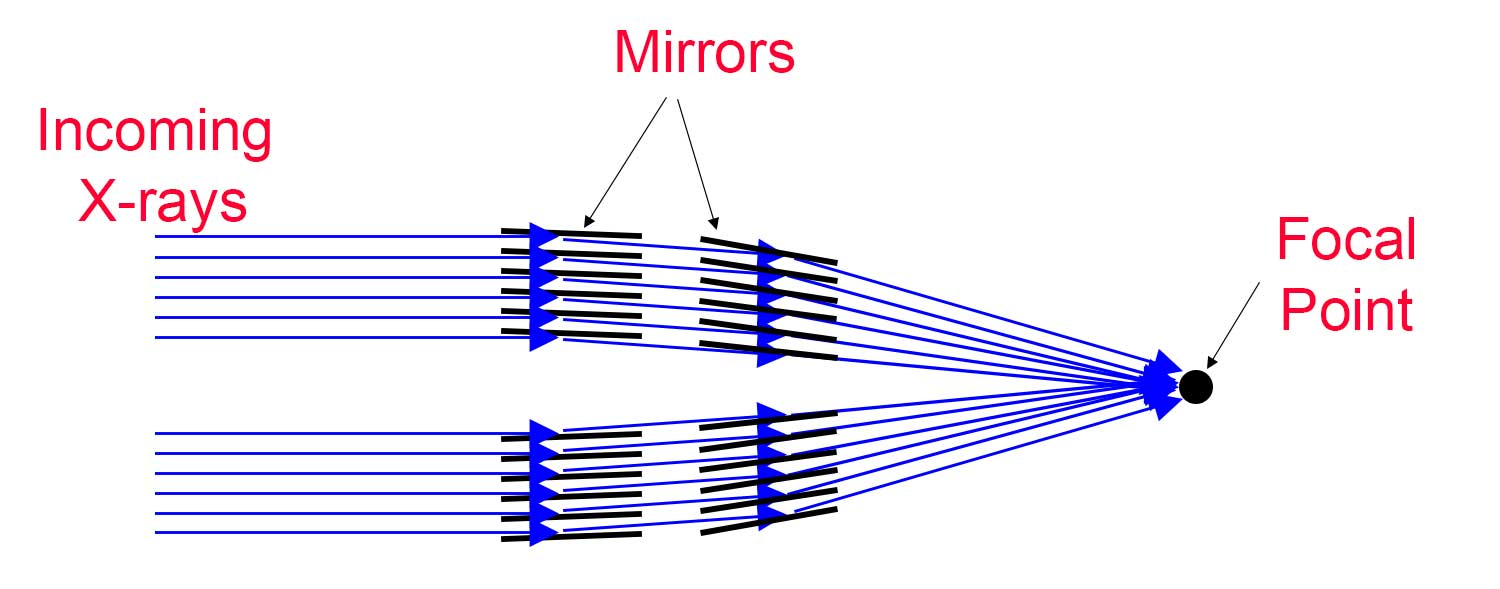
\includegraphics[width=0.7\linewidth]{Figures/xray_telescope_multimirror.jpg}
 \caption{Σχηματικό διάγραμμα κατά μήκος τομής τηλεσκοπίου ακτίνων Χ με αρκετά σετ κατόπτρων. Με ένθετα κάτοπτρα περισσότερες δέσμες εστιάζονται παρέχοντας λαμπρότερη απεικόνιση. (Εικόνα από το <<\textlatin{Imagine the Universe}>> της \textlatin{NASA})} \label{fig:multimirror}
 \end{center}
\end{figure*}

Τοποθετώντας τα κάτοπτρα στις εσωτερικές πλευρές του <<σωλήνα>> που αποτελεί τον κορμό του τηλεσκοπίου, υπάρχει ένα κενό στο κέντρο με αποτέλεσμα το τηλεσκόπιο να χάνει πολλές ακτίνες Χ. Για να λυθεί το πρόβλημα αυτό, τα τηλεσκόπια ακτίνων Χ χρησιμοποιούν κυλινδρικά κάτοπτρα και τα τοποθετούν ένθετα το ένα μέσα στο άλλο- όπως σχηματικά βλέπουμε στο σχήμα \ref{fig:multimirror}. Σημαντικό ρόλο παίζει το υλικό του κατόπτρου (υλικά με υψηλό ατομικό αριθμό Ζ ανακλούν καλύτερα υψηλοενεργειακά φωτόνια- για αυτό συχνά τα κάτοπτρα είναι επιχρυσωμένα) καθώς και η λείανση της κατοπτρικής επιφάνειας για να μην υπάρχουν σημαντικές απώλειες.

\begin{figure*}
 \begin{center}
 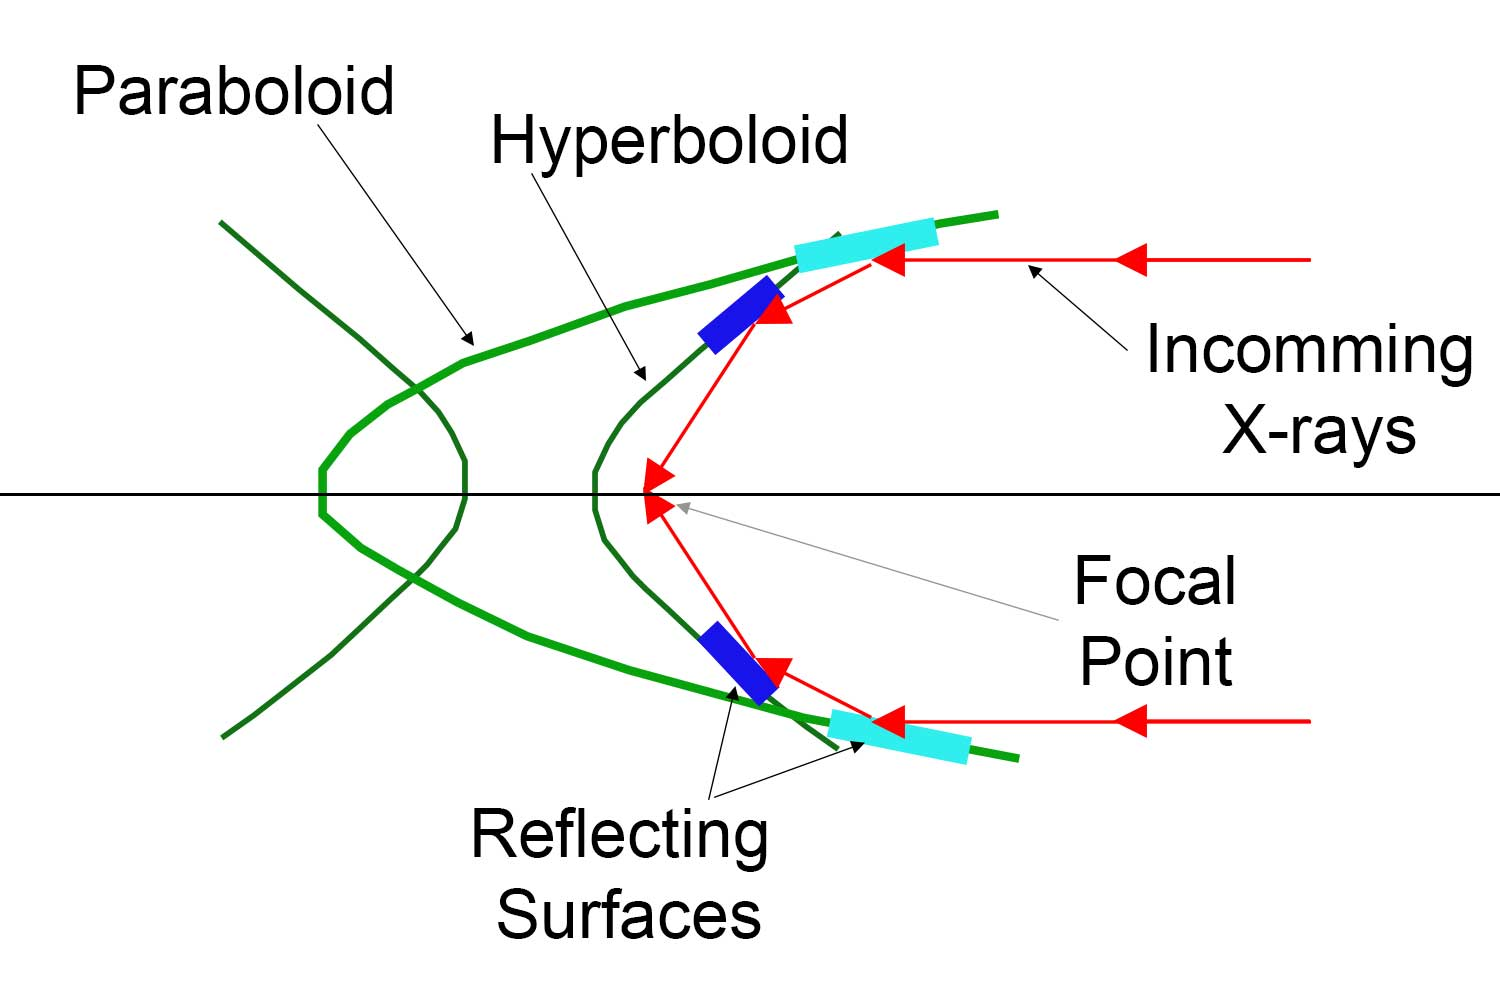
\includegraphics[width=0.7\linewidth]{Figures/wolter_typeI.jpg}
 \caption{Ο σχεδιασμός που ακολουθεί ένα τηλεσκόπιο \textlatin{Wolter} τύπου 1. Το παραβολοειδές εκ περιστροφής σχήμα των κατόπτρων και το υπερβολοειδές εκ περιστροφής σχήμα των κατόπτρων έχουν κοινό άξονα με την γραμμή παρατήρησης και κοινό εστιακό επίπεδο μεταξύ τους. (Εικόνα από το <<\textlatin{Imagine the Universe}>> της \textlatin{NASA})} \label{fig:wolter}
 \end{center}
\end{figure*} 

Η κατασκευή που χρησιμοποιείται ευρέως στην αστρονομία ακτίνων Χ και συγκεκριμένα στο τηλεσκόπιο \textlatin{XMM-Newton} λέγεται κάτοπτρο \textlatin{Wolter} τύπου 1 και είναι μια διαδοχή κατόπτρων υπερβολοειδούς σχήματος κοντά στο εστιακό επίπεδο που καταλήγουν σε παραβολοειδές σχήμα στην αντίθετη άκρη του τηλεσκοπίου- όπως φαίνεται στο σχήμα \ref{fig:wolter}. Η εικόνα σχηματίζεται στο εστιακό επίπεδο μετά από διαδοχική ολική ανάκλαση από την παραβολοειδή και την υπερβολοειδή επιφάνεια. Το σχήμα αυτό είναι μηχανικά απλό και επιτρέπει την τοποθέτηση πολλών κατόπτρων το ένα μέσα στο άλλο, αυξάνοντας έτσι την ωφέλιμη επιφάνεια ανάκλασης ώστε να έχουμε ευκρινείς παρατηρήσεις και καλές μετρήσεις για αμυδρές πηγές που δεν θα μπορούσαμε να παρατηρήσουμε διαφορετικά. 

\subsection{Το τηλεσκόπιο \textlatin{XMM-Νewton}}

Το \textlatin{XMM-Νewton} έχει τρία τηλεσκόπια ακτίνων Χ και ένα τηλεσκόπιο για οπτικό/ υπεριώδες.\\
Κάθε ένα από τα τρία τηλεσκόπια του \textlatin{XMM-Newton} αποτελείται από 58 ένθετα κάτοπτρα \textlatin{Wolter} τύπου 1 κατασκευασμένα ιδανικά για δέσμες που προσπίπτουν υπό γωνία ${0^ο} {30^\prime}$ με την επιφάνεια του κατόπτρου προσφέροντας, έτσι, υψηλή ανακλαστικότητα σε ακτίνες ενεργειών $\sim 7$ \textlatin{keV}. Το εστιακό μήκος των τηλεσκοπίων είναι $7.5$ \textlatin{m} και η διάμετρος του εξωτερικού κατόπτρου είναι $70$ \textlatin{cm}. Η διάρθρωση αυτή και το πλήθος των κατόπτρων καθιστούν το \textlatin{XMM-Newton} ένα από τα τηλεσκόπια ακτίνων Χ με την μεγαλύτερη ευαισθησία.
  
Το \textlatin{XMM-Newton} προσφέρεται για απεικόνιση ή απεικονιστική φασματοσκοπία που δεν απαιτεί διακριτική ικανότητα καλύτερη από $5$ \textlatin{arcsec} (στο σύστημα απεικόνισης του \textlatin{XMM-Newton} ένα \textlatin{pixel} αντιστοιχεί σε $4.4$ \textlatin{arcsec}) και για φασματοσκοπία υψηλής ανάλυσης για ενέργειες $0.2- 2$ \textlatin{keV} και για φασματοσκοπία εκτεταμένων αντικειμένων ($>10$ \textlatin{arcsec} και $< 1$ \textlatin{arcmin}).

\subsection{Ανιχνευτές στο \textlatin{XMM-Νewton}}
  
Το \textlatin{XMM-Νewton} έχει τα εξής όργανα καταγραφής επιστημονικών δεδομένων\cite{Handbook}: 
\begin{itemize}
    \item \textlatin{EPIC (European Photon Imaging Camera):} Τρείς κάμερες \textlatin{CCD} για απεικόνιση ακτίνων Χ, φασματισκοπία μέτριας ευκρίνειας και φωτομετρία ακτίνων Χ. Έχουμε δύο διαφορετικά είδη κάμερων \textlatin{EPIC}: \textlatin{MOS} και ΡΝ με 7 και 12 \textlatin{chip} αντίστοιχα. Το \textlatin{XMM-Νewton} φέρει δύο κάμερες \textlatin{MOS} και μία ΡΝ.
    \item \textlatin{RGS (Reflection Grating Spectrometer):}  Δύο όμοια φασματόμετρα για υψηλής ευκρίνειας φασματοσκοπική ανάλυση ακτίνων Χ και φασματο-φωτομετρία.
    \item \textlatin{ΟΜ (Optical Monitor):}  για απεικόνιση στο οπτικό/υπεριώδες και φασματοσκοπία πλεγματικού πρίσματος.
\end{itemize}

\begin{figure*}
 \begin{center}
 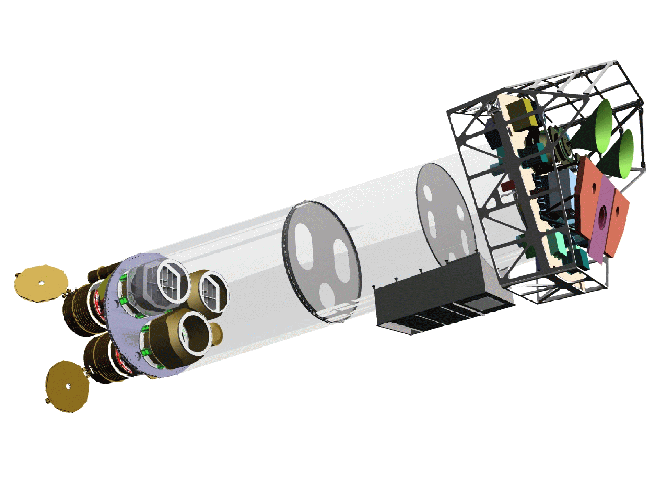
\includegraphics[width=0.9\linewidth]{Figures/img33.png}
 \caption{Σχηματικά τα μέρη που αποτελούν το παρατηρητήριο \textlatin{XMM}. Στο αριστερό άκρο, όπως φαίνεται στο σχήμα, οι τρείς μονάδες με τις συστάδες ένθετων κατόπτρων- οι δύο από τις οποίες έχουν πλεγματικά φράγματα (\textlatin{gratings}). Στο αντίθετο άκρο του παρατηρητηρίου φαίνονται τα όργανα στα εστιακά επίπεδα των τηλεσκοπίων: οι μηχανισμοί ψύξης των δύο κάμερων \textlatin{EPIC MOS} (οι δομές με μαύρο και πράσινο χρώμα), ο μηχανισμός ψύξης της \textlatin{EPIC} ΡΝ (με ανοιχτό μωβ χρώμα), οι ανιχνευτές \textlatin{RGS} (με φωτεινό γαλάζιο χρώμα) και οι μηχανισμοί ψύξης των \textlatin{RGS} (με κοκκινο-ροζ χρώμα)- δεν φαίνεται το οπτικό τηλεσκόπιο ΟΜ (βρίσκεται πίσω από την χαμηλότερη μονάδα ένθετων κατόπτρων στα αριστερά) (Εικόνα από το <<\textlatin{XMM-Newton User's Handbook, 2021.}>> \textlatin{ESA: XMM-Newton SOC})}
 \label{fig:XMMsketch}
 \end{center}
 \end{figure*}

Οι τρείς κάμερες \textlatin{EPIC} και οι δύο ανιχνευτές των φασματόμετρων \textlatin{RGS} βρίσκονται στα εστιακά επίπεδα των τηλεσκοπίων ακτίνων Χ, ενώ το ΟΜ στο τηλεσκόπιο οπτικού/υπεριώδους του παρατηρητηρίου \textlatin{XMM.} Ένα σχέδιο του παρατηρητηρίου \textlatin{XMM} φαίνεται στο σχήμα \ref{fig:XMMsketch}. Τα επιστημονικά όργανα του \textlatin{XMM} μπορούν να λειτουργούν ταυτόχρονα αλλά και αυτόνομα σε διαφορετικές καταστάσεις λειτουργίας.\\
Οι κάμερες \textlatin{EPIC} λειτουργούν ως καταμετρητές φωτονίων \textlatin{(photon counting mode)} με σταθερή συχνότητα  \textlatin{read-out} παράγοντας λίστες γεγονότων (πίνακες με μία γραμμή για κάθε καταχώρηση γεγονότος που περιλαμβάνει, μεταξύ άλλων, τα χαρακτηριστικά του γεγονότος όπως θέση, χρονική στιγμή καταγραφής και ενέργεια.)\\ 
\begin{figure*}
 \begin{center}
 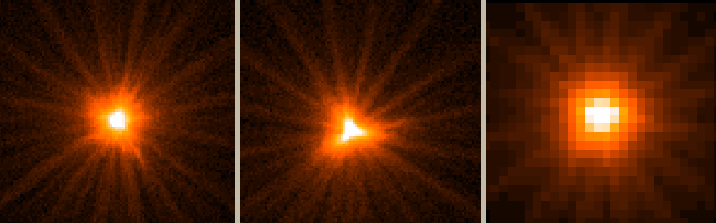
\includegraphics[width=0.9\linewidth]{Figures/PSFs.png}
 \caption{Η συνάρτηση εξάπλωσης σημείου \textlatin{PSF} για τους ανιχνευτές \textlatin{MOS1}, \textlatin{MOS2} και ΡΝ (από τα αριστερά στα δεξιά) για την ίδια πηγή στις ακτίνες Χ. Το μέγεθος \textlatin{pixel} αντιστοιχεί σε $1.1\; arcsec$ για τους ανιχνευτές \textlatin{MOS} και σε $4.1\;arcsec$ για τον ανιχνευτή ΡΝ (Εικόνα από το <<\textlatin{XMM-Newton User's Handbook, 2021.}>> \textlatin{ESA: XMM-Newton SOC})}
 \label{fig:PSFs}
 \end{center}
 \end{figure*}
\begin{figure*}%
    \centering
    \subfloat{{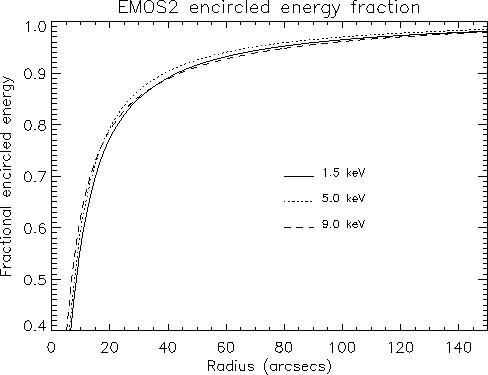
\includegraphics[width=0.46\linewidth]{Figures/EFF_M1.png} }}%
    \qquad
    \subfloat{{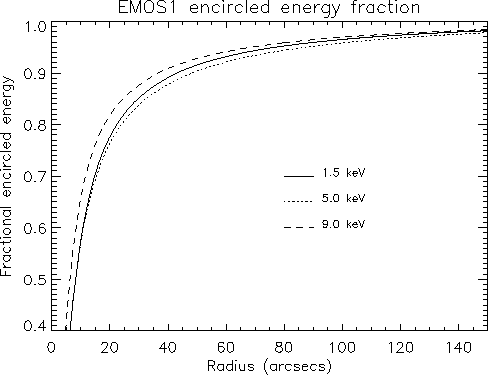
\includegraphics[width=0.46\linewidth]{Figures/EFF_M2.png} }}%
     \caption{Το κλάσμα ενεργειακής ισχύος που περικλείεται στην παρατήρηση σε συνάρτηση με την γωνιακή ακτίνα του διαφράγματος στον άξονα παρατήρησης για ακτινοβολίες διαφορετικών ενεργειών. Αριστερά: για τον ανιχνευτή \textlatin{EPIC MOS1}. Δεξιά: για τον ανιχνευτή \textlatin{EPIC MOS2}. (Εικόνα από το <<\textlatin{XMM-Newton User's Handbook, 2021.}>> \textlatin{ESA: XMM-Newton SOC})} \label{fig:EEF_MOS}
\end{figure*}
\begin{figure*}
 \begin{center}
 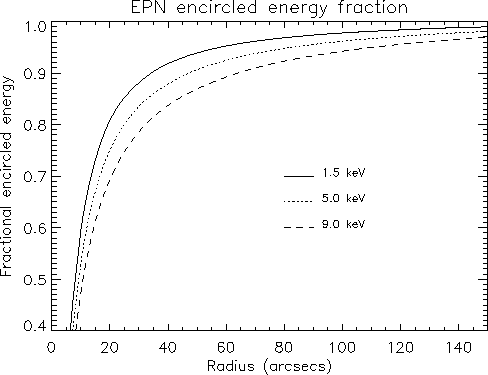
\includegraphics[width=0.7\linewidth]{Figures/EFF_PN.png}
 \caption{Το κλάσμα ενεργειακής ισχύος που περικλείεται στην παρατήρηση σε συνάρτηση με την γωνιακή ακτίνα του διαφράγματος στον άξονα παρατήρησης για ακτινοβολίες διαφορετικών ενεργειών για τον ανιχνευτή \textlatin{EPIC} ΡΝ. (Εικόνα από το <<\textlatin{XMM-Newton User's Handbook, 2021.}>> \textlatin{ESA: XMM-Newton SOC})}
 \label{fig:EEF_PN}
 \end{center}
 \end{figure*}
Η γωνιακή ικανότητα των ανιχνευτών \textlatin{EPIC} καθορίζεται από την συνάρτηση εξάπλωσης σημείου \textlatin{PSF} η οποία με την σειρά της καθορίζεται από τα κάτοπτρα (σχήμα \ref{fig:PSFs}). Οι \textlatin{EPIC MOS} και ΡΝ έχουν \textlatin{pixel} μεγέθους $40$ και $150$ m\textlatin{m} αντίστοιχα. Για το εστιακό μήκος των τηλεσκοπίαν ($7.5$ \textlatin{m}) αυτό αντιστοιχεί σε $1.1\; arcsec$ στον ουράνιο θόλο για τις \textlatin{EPIC MOS} και $4.1$ \textlatin{arcsec} για την \textlatin{EPIC PN}.\\
Ανάλογα με την γωνιακή ακτίνα του διαφράγματος, διαφορετικό ποσοστό της ροής σημειακής πηγής (δηλαδή της \textlatin{PSF}) περικλείεται στην παρατήρηση. Στα σχήματα \ref{fig:EEF_MOS} kai \ref{fig:EEF_PN} χαράσεται η συναρτησιακή αυτή σχέση για κάθε ανιχνευτή ξεχωριστά. 

Οι παρατηρήσεις των στοχευμένων \textlatin{(pointed)} πηγών έγιναν με άνοιγμα διάφραγματος ακτίνας $15$ \textlatin{arcsec} ενώ για παρατηρήσεις πηγών κατά την περιστροφή του τηλεσκοπίου \textlatin{(slew)} η ακτίνα του διάφραγματος είναι $30$ \textlatin{arcsec}\cite{RapidXMM}.
H καταγραφή του υποβάθρου γίνεται με μία μάσκα δακτυλιοειδούς σχήματος με εσωτερική ακτίνα $60$ \textlatin{arcsec} και εξωτερική ακτίνα $180$ \textlatin{arcsec}, η μάσκα αυτή επιτρέπει το άνοιγμα του διαφράγματος να περιορίζεται σε δακτύλιο μεταξύ των ακτίνων αυτών για τον υπολογισμό του υποβάθρου και προσαρμόζεται στην κλίμακα κάθε παρατήρησης πολλαπλασιάζοντας με τον λόγο των εμβαδών του διαφράγματος έκθεσης\cite{RapidXMM}. 

\subsubsection*{Απόδοση των ανιχνευτών ακτίνων Χ}

\begin{figure*}
 \begin{center}
 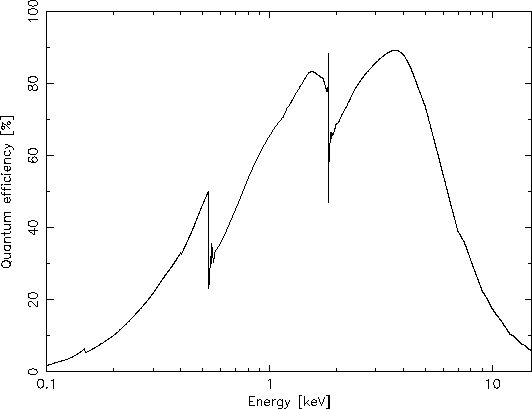
\includegraphics[width=0.7\linewidth]{Figures/mosqe.png}
 \caption{Η κβαντική απόδοση των \textlatin{chip} των ανιχνευτών \textlatin{EPIC MOS} ως συνάρτηση της ενέργειας των φωτονίων. (Εικόνα \cite{MOS})}
 \label{fig:QE_mos}
 \end{center}
 \end{figure*}
\begin{figure*}
 \begin{center}
 
\includegraphics[width=0.7\linewidth]{Figures/pnqe.png}
 \caption{Η κβαντική απόδοση των \textlatin{chip} των ανιχνευτών \textlatin{EPIC} ΡΝ ως συνάρτηση της ενέργειας των φωτονίων.(Εικόνα \cite{PN})}
 \label{fig:QE_pn}
 \end{center}
 \end{figure*}
Ένας παράγοντας που πρέπει να ληφθεί υπ>όψιν για την απόδοση των ανιχνευτών \textlatin{EPIC} είναι η κβαντική απόδοση των \textlatin{chip} των ανιχνευτών που περιορίζει τις ενέργειες που μελετάμε.
Όπως βλεπουμε στα σχήματα \ref{fig:QE_mos} kai \ref{fig:QE_pn}, τα \textlatin{chip} του ανιχνευτή ΡΝ έχουν απόδοση από $0.6-1.0$ στο ενεργειακό παράθυρο $0.15-2.0$ \textlatin{keV}, απόδοση σχεδόν 1 στο ενεργειακό παράθυρο $2.0-9.0$ \textlatin{keV} kai απόδοση $0.6-0.9$ για ενέργειες $10-15$ \textlatin{keV}, αντίθετα τα \textlatin{chip} των ανιχνευτών \textlatin{MOS} δεν έχουν συστηματικά πολύ μεγάλη απόδοση σε μεγάλο εύρος ενεργειών.

\subsection{Παρατηρήσεις του \textlatin{XMM-Νewton}}

\begin{figure*}%
    \centering
    \subfloat{{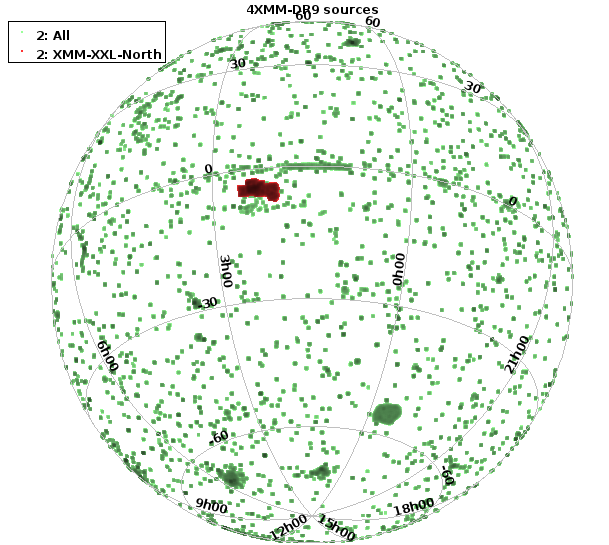
\includegraphics[width=0.46\linewidth]{Figures/4XMM-DR9 sources.png} }}%
    \qquad
    \subfloat{{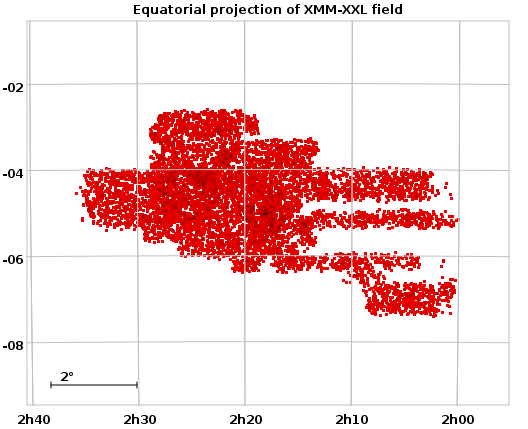
\includegraphics[width=0.46\linewidth]{Figures/EquatorialViewXMMXXL.png} }}%
     \caption{Αριστερά: Ισημερινή προβολή των πηγών που έχει καταγράψει το \textlatin{XMM-Newton} είτε στοχευμένα (\textlatin{pointed}) είτε κατά την περιστροφή του τηλεσκοπίου (\textlatin{slew}), το πεδίο \textlatin{XMM-XXL-North} απεικονίζεται με διαφορετικό χρώμα. Δεξιά: προβάλονται οι πηγές με στοχευμένες παρατηρήσεις του πεδίου \textlatin{XMM-XXL-North} σε ισημερινή προβολή. Ο οριζόντιος άξονας είναι η διορθωμένη για ιδία κίνηση ορθή αναφορά (\textlatin{RA}) και ο κατακόρυφος άξονας η διορθωμένη απόκλιση (\textlatin{Dec}). (Οι παραπάνω εικόνες παρήχθησαν χρησιμοποιώντας το πρόγραμμα απεικόνισης \textlatin{TOPCAT} \cite{TopCat} και τους καταλόγους \textlatin{4XMM-DR9}\cite{2020yCat.9059....0W} kai \textlatin{RapidXMM} \cite{RapidXMM})} \label{fig:XMMfield}
\end{figure*}
  
To \textlatin{XMM-Νewton} έχει συμμετάσχει σε πολλές έρευνες, έχει καλύψει πεδία που έχουν παρατηρηθεί ήδη από άλλα τηλεσκόπια και έχει λάβει δεδομένα τόσο με στοχευμένες (\textlatin{pointed}) παρατηρήσεις όσο και κατά την περιστροφή του (\textlatin{slew}). Ως μέρος της έρευνας \textlatin{XMM-XXL}, χαρτογραφήθηκαν από το \textlatin{XMM-Νewton} δύο νέα πεδία: το \textlatin{XMM-XXL-North} kai to \textlatin{XMM-XXL-South}, τα οποία καλύπτουν συνδυαστικά $\sim 50 $ \textlatin{deg}$^2$. Στην εικόνα \ref{fig:XMMfield} βλέπουμε μία άποψη από όλες τις παρατηρήσεις του \textlatin{XMM-Νewton} (με πράσινο χρώμα) στον ουράνιο θόλο, ενώ με κόκκινο σημειώνεται το πεδίο \textlatin{XMM-XXL-North}. Το πεδίο \textlatin{XMM-XXL-North} (με κόκκινο χρώμα στην εικόνα \ref{fig:XMMfield} αποτελεί το πεδίο στο οποίο στηρίζεται η παρούσα εργασία.
%με κοκκινο το ΧΜΜ-ΧΧΛ, που αποτελει και το βασικο πεδιο πανω στο οποιο στηριζεται η παρουσα εργασια. 
  
  
  
  
  
  
  
  
  
  
